%%%%%%%%%%%%%%%%%%%%%%%%%%%%%%%%%%%%%%%%%%%%%%%%%%%%%%%%%%%%%%%%%%%%%%%%%%%
% filename    : sp.tex
% author      : 
%%%%%%%%%%%%%%%%%%%%%%%%%%%%%%%%%%%%%%%%%%%%%%%%%%%%%%%%%%%%%%%%%%%%%%%%%%%

% BUGFIX: Save LaTeX kernel version of \@xfloat
\makeatletter
\let\my@xfloat\@xfloat
\makeatother

% use ateneo de naga etd class (actually modified virginia tech's etd class)
\documentclass[oneside]{etd}

% BUGFIX: Create a modified copy of \@xfloat using the kernel definition
\makeatletter
\def\@xfloat#1[#2]{
	\my@xfloat#1[#2]%
	\def\baselinestretch{1}%
	\@normalsize \normalsize
}
\makeatother

% use these packages

\usepackage{array}
\usepackage{graphicx}
\usepackage{amssymb}
\usepackage{gensymb}
\usepackage{latexsym}
\usepackage{amsmath}
\usepackage{booktabs}
%\usepackage[lineno5,noindent]{lgrind}
%\usepackage{rotating} 
%\usepackage{makeidx}
%\usepackage{stmaryrd}
\usepackage{float}
\usepackage{subfigure}
\usepackage{amssymb}
\usepackage{longtable}
\usepackage{hyperref}
\usepackage[numbers]{natbib}
%\usepackage{cite}
%\usepackage{moreverb}
%\usepackage{pictexwd,dcpic}
\usepackage{algorithm,algorithmic}
\renewcommand{\algorithmicrequire}{\textbf{Input:}}
\renewcommand{\algorithmicensure}{\textbf{Output:}}
\usepackage{tikz}
\usetikzlibrary{positioning,calc}

\usepackage{graphicx}

\newcommand{\pandocbounded}[1]{#1}

\usepackage{listings}
\definecolor{cppred}{rgb}{0.6,0,0} % for strings
\definecolor{cppgreen}{rgb}{0.25,0.5,0.35} % comments
\definecolor{cpppurple}{rgb}{0.5,0,0.35} % keywords
\definecolor{cppdocblue}{rgb}{0.25,0.35,0.75} % doc

% Fix for \tightlist undefined error
\providecommand{\tightlist}{%
  \setlength{\itemsep}{0pt}\setlength{\parskip}{0pt}}

\lstset{language=C++,
basicstyle=\linespread{0.8}\ttfamily\small,
keywordstyle=\color{cpppurple}\bfseries,
stringstyle=\color{cppred},
commentstyle=\color{cppgreen},
morecomment=[s][\color{cppdocblue}]{/**}{*/},
numbers=left,
numberstyle=\tiny\color{black},
% stepnumber=2,
numbersep=10pt,
tabsize=4,
showspaces=false,
showstringspaces=false}

\graphicspath{{figures/}{./}}

%\renewcommand{\floatpagefraction}{0.8}

\makeindex

%%%%%%%%%%%%%%%%%%%%%%%%%%%%%%%%%%%%%%%%%%%%%%%%%%%%%%%%%%%%%%%%%%%%%%%%%%%

\title{Formal Specification and Behavioural Analysis of the Inter-Blockchain Communication Protocol: Are Asset Transfer and Data Transport Semantically Unified, Stacked, or Conflicting?}
\department{Computer Science}
\BSthesis % options: \BSthesis \BSproject \BShonors \Mdegree \MSdegree \PhDdegree
\degreemonth{25 May}  % date of final defense
\degreeyear{2026}

\twostudents % options: \onestudent \twostudents \threestudents \fourstudents
{Jazztine Kirvy Gonzales}
{Jonel C. Ganalon}

\studentsheader
{Gonzales, Ganalon}

\twodegrees % options: \onedegree \twodegrees \threesdegrees \fourdegrees
{Computer Science}
{Computer Science}

\advisor
{Adviser's Name}
\threemembers
{First Panel Member}
{Second Panel Member}
{Third Panel Member}
\deanandchair
{Joshua Martinez}
{Lowie Vincent Bisana, MIT}

\keywords{Blockchain, Interoperability, Semantics, IBC, Process Algebra}

\begin{document}

%edit etd.cls to accommodate lesser number of proponents
\maketitle
\makerecomm
\makeacceptance
\makedeclaration

%%%%%%%%%%%%%%%%%%%%%%%%%%%%%%%%%%%%%%%%%%%%%%%%%%%%%%%%%%%%%%%%%%%%%%%%%%%
%                    ABSTRACT/EXECUTIVE SUMMARY                           %
%%%%%%%%%%%%%%%%%%%%%%%%%%%%%%%%%%%%%%%%%%%%%%%%%%%%%%%%%%%%%%%%%%%%%%%%%%%

% can use execsummary or abstract
\begin{abstract}
The Inter-Blockchain Communication (IBC) protocol is the most widely adopted interoperability solution, enabling over 100 heterogeneous blockchains to exchange both digital assets and arbitrary data. However, a fundamental question remains unanswered: Are IBC's asset-transfer (ICS-020) and data-transport (ICS-004) behaviours semantically unified, stacked, or conflicting? This research provides the first formal specification and behavioural analysis of IBC using process algebra and labelled transition systems (LTS). Unlike prior trace-based formalisations using TLA\textsuperscript{+} , process algebra preserves branching structure, concurrent composition, and silent abstraction which are essential for detecting behavioural anomalies. The research produces complete process algebra specifications of ICS-004 and ICS-020, extracts LTS models via structural operational semantics, and compares observable behaviours using weak bisimulation and deadlock analysis. The three analytical scenarios are operationally defined: unified (weak bisimilarity), stacked (trace inclusion without bisimilarity), or conflicting (emergent deadlocks under parallel composition). The methodology follows five phases: domain analysis, process algebra specification, LTS extraction, behavioural comparison, and reusable documentation. Findings will provide developers, auditors, and chain operators with mathematically grounded assurance of IBC's semantic interoperability, while establishing a reusable formal framework for comparing other protocols such as Polkadot XCM and Axelar. This work addresses critical gaps in blockchain interoperability theory: no prior formal comparison of asset versus data behaviours, no process-algebraic treatment of IBC semantics, and no operational criteria for unified-stacked-conflicting classification.
\end{abstract}

\include{misc/dedication}
\begin{acknowledgements}

We thank everyone who helped me finish this thesis.

\end{acknowledgements}


\begingroup
\renewcommand*{\addvspace}[1]{}
\tableofcontents
\listoffigures
\listoftables
\endgroup

\beginbody
\pagenumbering{arabic}

\chapter{Introduction}\label{introduction}

After the inception of blockchain as a distributed ledger in 2009 with
the invention of Bitcoin, the concept of \textbf{blockchain
interoperability (BI)} soon followed and started to receive attention
\citep{Belchior_2021}. It is the ability of different blockchain
networks to communicate and exchange data, or currency and assets
without needing a centralised arbiter
\citep{kishore2025interoperability}. This is motivated by the
realisation that blockchains have become isolated silos or systems
incapable of communicating with their outside environment.
Interoperability permits technology to develop beyond its limitation to
scalability, reduces fragmentation in the ecosystem, and increases the
use of liquidity in different platforms \citep{belenkov2025review}
\citep{Saleh2024}. Without this, innovation will remain limited as
digital assets and information remain stagnant and isolated within their
own blockchain networks.

The early protocols for BI started development within 2015-2016. They
are mainly focused on the atomic exchanage of digital asset or tokens
between different networks
\citep{wilson2026exploringblockchaininteroperabilityframeworks}. These
protocols, such as sidechains, notary schemes, and hashed time-lock
contracts (HTLC), are categorised as \textbf{asset-based} since their
original goal is to facilitate the exchange of value and cryptocurrency
through an autonomous and synchronised way \citep{wang2021sok}.

When the blockchain usage moved beyond cryptocurrency to complicated
applications like provenance, tracking, and Internet of Things (IoT),
new protocols aimed to handle arbitrary data evolved \citep{Kotey_2024}.
As data from many applications quickly grow in volume, the need to
prioritise sharing arbitrary information and state transitions between
networks has become more evident \citep{wang2021sok}
\citep{kishore2025interoperability}. Since the earlier blockchains are
treated as isolated silos, the mere exchange of value is insufficient
for sectors like supply chain and healthcare that need wider
coordination and sharing of information
\citep{wilson2026exploringblockchaininteroperabilityframeworks}
\citep{madine2021appxchain}. This need led to the creation of
cross-blockchain smart contracts and messaging frameworks allowing
decentralised applications (dApps) to coordinate and verify information
from different chain without undergoing a centralised arbiter
\citep{Belchior_2021}.

Recognising the limitations of single-purpose protocols, developers
created unified interoperability protocols capable of handling both
assets and arbitrary data. The \textbf{Interblockchain (IBC)} protocol
is the leading example of this. It handles both digital assets and
arbitraty data by means of its payload-agnostic design; information is
delivered as byte-encoded packets whatever it contains
\citep{cosmos2024ibcintro} \citep{goes2020interblockchain}. This works
by separating the transport layer (TAO) (that focuses on transportation,
authentication, and arrangment of data) and the application layer (that
gives meaning to each payload) \citep{ibc2025howworks}.

For assets, IBC uses guidelines like (InterChain Standards) ICS-20 for
locking the original asset and minting the corresponding vouchers in the
target blockchain \citep{quasar2023litepaper}
\citep{ibc2024transportapp} \citep{goes2020interblockchain}. Meanwhile
for arbitrary data and application logic, ICS-27 (Interchain Accounts)
and ICS-31 (Interchain Queries) are used in order to execute commands or
read states from other network without needing a centralised arbiter
\citep{quasar2023litepaper} \citep{ibc2024transportapp}. IBC serves as a
general-purpose communication layer similar to TCP/IP of the Internet
that allows heterogenous blockchains to exchange whatever type of
information in a way that is safe and trust-minimised.

\section{Project Context}\label{project-context}

The \textbf{Inter-Blockchain Communication (IBC) Protocol} is considered
as the most used and widely adopted interoperability protocol that can
handle both digital assets and arbitrary data
\citep{ibc2024transportapp} \citep{Belchior_2021}. As a general-purpose
message-passing protocol, it serves as the connective tissue of more
than 100 different blockchains (where 107 chains uses reference
implementation of IBC-Go) to cooperate in a way that is secure,
permissionless, and trust-minimised. Its payload-agnostic design enables
it to deliver whatever information that is encoded in bytes --- from
simple token transfers using ICS-20 standard to more complex arbitrary
data and application logic like ICS-27 (Interchain Accounts) and ICS-31
(Interchain Queries). Because of its wide adoption and ability to serve
as a universal standard like TCP/IP of Internet, it is the leading
solution in creating an Internet of Blockchains that supports different
workflows in the whole ecosystem \citep{kishore2025interoperability}.

However, despite IBC\textquotesingle s widespread adoption, a
fundamental question remains unanswered: Do IBC\textquotesingle s
asset-transfer and data-transfer behaviours share the same core
semantics (unified), are assets semantics merely built on top of data
transport without fundamental integration (staked), or do these
behaviours interfere with each other in ways that create observable
anomalies (conflicting)?

\textbf{Semantic interoperability}, or the ability of different
blockchain networks to understand exchanged data and use it meaningfully
in their own systems, depends on answering this question
\citep{Saleh2024} \citep{Belchior_2021}. Without a clear understanding
of how asset and data behaviours relate within a unified protocol like
IBC, developers cannot be certain that cross-chain operations will
behave predictably. At the same time, auditors cannot guarantee that
security properties hold across both asset transfers and arbitrary
message passing.

\textbf{Formal modelling} answers the problem of semantic
interoperability by providing a mathematical and clear description of
the characteristics of the systems that removes ambiguity or
misconceptions on how data should be understood and processed
\citep{verma2022formalmethods}. It serves as the foundation in ensuring
that application-specific semantics are maintained amidst the
differences in architecture and consensus mechanisms \citep{Saleh2024}
\citep{Belchior_2021}. Formal verification like model checking, provides
irrefutable evidence to the developers and auditors that the
coordination of the behaviours of assets and arbitrary data remain
predictable and safe within a unified protocol like the IBC.

Currently, formalisation on IBC is focused on its TAO using tools like
TLA+ in order to verify the correctness, safety, and liveness of its
protocol \citep{Wei_2023}. There is a need to formalise its semantic
interoperability layer because although ICS dictates guidelines for
applications, there is insufficient mathematical foundation that
verifies the coordination of the behaviours of assset and arbitrary data
within system.

This research will use \textbf{Process Algebra} to model the behaviour
of IBC protocol.

\section{Purpose and Description}\label{purpose-and-description}

The main purpose of this research is to formally specify and analyse the
observable behaviours of the IBC protocol using process algebra and
labelled transition systems (LTS). Specifically, this research will:

\begin{enumerate}
\tightlist
\item
  Produce the first complete process algebra specification of
  IBC\textquotesingle s core protocols (ICS-004 for data transport and
  ICS-020 for asset transfer).
\item
  Extract LTS behavioural models from these specifications.
\item
  Analyse whether IBC\textquotesingle s asset-transfer and data-transfer
  behaviours are unified, stacked, or conflicting.
\end{enumerate}

Unlike the prior formal analyses of IBC using TLA+ trace-based
verification, this research uses process algebra which is a formalism
uniquely suited to capturing concurrent interaction, branching
structure, and silent abstraction. This provides a complementary
perspective that can reveal behavioural anomalies that trace-based
methods might miss.

Aside from developers and auditors, this will give dApp developers
assurance and predictability in developing ccross-chain applications.
For chain operator and validator, this will reduce development risk and
ensures stability of the system against dynamic runtime errors like
deadlock or livelock \citep{Kotey_2024} \citep{Duan2018}. Lastly,
end-users can ensure the integrity and security of their asset and
transaction in a trust-minimised environment \citep{Kotey_2024}.

To guide this research, the following questions are posed:

\begin{enumerate}
\tightlist
\item
  How can IBC (including both asset transfer and data transfer) be
  formally specified using process algebra?
\item
  What obervable behaviours (traces, ordering constraints, branching
  structure, deadlocks, synchronisation patterns) emerge from the LTS
  model of IBC?
\item
  Within the IBC specification, are the behavioural patterns for asset
  transfer and data transfer: a. Unified (they share the same core
  semantics)? b. Stacked (asset semantics are built on top of data
  transport without fundamental integration?) c. Conflicting (they
  interfere with each other in ways that cause observable behavioural
  anomalies?)
\end{enumerate}

\section{Objectives}\label{objectives}

To achive the main purpose of this research, the following specific
objectives must be accomplished:

\begin{enumerate}
\tightlist
\item
  Identify and define the atomic actions, alphabets, communication
  ports, and data types necessary to model IBC\textquotesingle s ICS-004
  and ICS-020 in process algebra.
\item
  Formally specify IBC\textquotesingle s core interaction patterns using
  process algebra operators.
\item
  Extract LTS models from the process algebra specifications, capturing
  all reachable states and observable transitions.
\item
  Analyse the LTS models to identify traces, ordering constraints,
  branching structures, deadlock states, and synchrnisation pattern for
  both asset-transfer and data-transfer scenarios.
\item
  Compare the behavioural patterns for asset transfer and data transfer
  within IBC specification to determine whether they are unified,
  stacked, or conflicting.
\item
  Document the process algebra specification and LTS models in a
  reusable form suitable for future comparative studies with other
  interoperability protocols like Polkadot XCM and Axelar.
\end{enumerate}

\section{Scope and Limitations}\label{scope-and-limitations}

The formal model abstracts away low-level details such as cryptographic
verification (Merkle proofs), light client synchronisation, and relayer
behaviour

Economic incentives (gas costs, slashing, liquidity constraints) are not
modelled

The analysis focuses on observable behaviour only; security properties
beyond what is observable (e.g., double-spending resistance) are not
verified

Only IBC\textquotesingle s core ICS-004 and ICS-020 standards are
modelled; other application standards (ICS-27, ICS-31) are excluded

No empirical validation or actual protocol instance execution is
performed

\chapter{Review of Related
Literature}\label{review-of-related-literature}

In the current landscape of blockchain technology, the emergence of
heterogeneous networks has revealed the term "information isolated
isalands" or "value silos" \citep{wang2021sok} \citep{Bigiotti2025}
\citep{Wu_2023}. Although individual blockchains proved to be useful as
independent ledgers, the lack of communication between them limits their
potential widespread adoption \citep{Hassan_2025} \citep{Cheng_2024}
\citep{Lohachab_2021}. Blockchain interoperability then becomes a
critical interaction between distributed systems \citep{wang2021sok}
\citep{Li2025} \citep{Lohachab_2021}.

Blockchain systems have been described as an independent state machine
with its own concensus rules and encryption standards
\citep{Bigiotti2025} \citep{Belchior_2021}. Because they do not have a
shared state or global clock between them, their interactions must
happen asynchronously; they must instead use message passing and state
synchronisation \citep{wang2021sok} \citep{Wei_2023}. In other words,
blockchain interoperability is a process wherein one source chain is
trying to change the state of a target chain by means of delivering
information or assets under certain securoty assumptions
\citep{wang2021sok} \citep{Wang_2023} \citep{belchior2021survey}.

Most of study in the literature focus on the blockchain interoperability
architecture. That is, whether it uses relays, sidechains, or notaries
\citep{Kotey_2023} \citep{Caetano_da_Silva_2025} \citep{Li_2023}
\citep{Chen_2023}. Nevertheless, recent studies have put emphasis that
architecture only gives stucture and real security and effectiveness of
interoperability depends on the behaviour of the system
\citep{Llambas2025} \citep{Llambas2024eventb} \citep{Lohachab_2021}.
This behaviour dictates how systems guarantee ACID (atomicity,
consistency, isolation, durability) properties in an asynchronous
network \citep{wang2021sok} \citep{Bigiotti2025} \citep{Wang_2023}
\citep{Li2025}.

This means that the sequencing of state transitions, timing of
cyrptographic proofs, and reactions to failure or timeout reveals the
system\textquotesingle s behaviour \citep{Ou_2022}
\citep{Chervinski_2023} \citep{deng2025} \citep{Wei_2023}.The analysis
of behaviours, instead of the static design, gives deeper understanding
on how different components (such as smart contracts and relayers)
interact during different processe. That is so to achieve semantic
interoperability where the meaning and context of data or asset from the
source chain gets accurately interpreted and valid to the target chain
\citep{Belchior_2023} \citep{sottomayor2024enterprise} \citep{Li2025}.

\section{Evolution of Blockchain
Interoperability}\label{evolution-of-blockchain-interoperability}

Surveying the literature, it is noticeable that the classifications of
interoperability reflects the underlying logic on how to trust and treat
information between blockchains \citep{wang2021sok} \citep{Pillai_2022}
\citep{wang2023}. Although categorical labels like notary schemes,
sidechains/relays, and hash-locking are usually used, there is a deeper
abstraction that surfaces in recent literature. That is, the perspective
of looking at blockchain interoperability as a multi-layered problem
derived from the OSI model of the internet \citep{Hassan_2025}
\citep{deng2025}.

The common abstraction from most of the sources is the
\textbf{source-target model}. In this model, an operation from the
source chain needs to trigger a corresponding state change to the target
chain \citep{deng2025} \citep{Cheng_2024}. The following differentiates
a critical difference on how this interaction gets seen:

\begin{itemize}
\item
  \textbf{Interoperability as Transfer:} In this perspective, the logic
  focuses on migration or transfer of ownership. Every transaction must
  follow all-or-nothing atomicity in order to avoid double-spending
  \citep{wang2021sok} \citep{Llambas2024patterns} \citep{deng2025}.
  Asset-based protocols belong here, ensuring that the value will not
  vanish or gets duplicated between different silos
  \citep{Belchior_2023} \citep{wang2023}.
\item
  \textbf{Interoperability as Communication:} In this perspective, the
  system gets treated as a \textbf{message-oriented service}
  \citep{wang2021sok} \citep{Kotey_2023} \citep{kang2022}. The goal is
  not to transfer the content of the source chain but to invoke a
  functionality in the target chain using arbitrary data
  \citep{Pillai_2022} \citep{Belchior_2021}. This is the logic of the
  data-based protocols like Arbitrary Message Passing (AMP)
  \citep{augusto2025}.
\end{itemize}

It is critical to make the distinction between asset-based and
data-based interoperability because they usually remain implicit in a
number of older literature. For instance, in the classical SoK
(Systematisation of Knowledge) of Buterin, the focus was always in value
exchange or value islands \citep{wang2021sok} \citep{A_Alzahrani_2025}
\citep{Pillai_2022}. However, in the newer frameworks, there is an
explicit division in the domain between \textbf{Asset Interoperability}
(migration/exchange) and \textbf{Data Interoperability} (cross-chain
calls/integration) \citep{deng2025} \citep{Cheng_2024} \citep{Li2025}.
This gap is important as a number of current models are designed for
assets but gets applied to data or vice-versa without taking each
different semantic requirements into consideration \citep{Belchior_2023}
\citep{Li2025}.

This differeng individual trust boundary and security assumptions of
each approaches contributes to the fragmented landscape of blockchain
interoperability\citep{Belchior_2023}. Although there is an attemot to
have a Generic Interoperability Paradigm comprising of Setup, Commit,
Verify, and Abort phases, the literature has not fully explained how
these phases differ in their \textbf{observable behaviour} when assets
are passed isnstead of arbitrary data \citep{deng2025} \citep{Li2025}.
This forms the need of a \textbf{comparative semantic analysis} to see
if these models are enough to encompass the behaviour of both asset and
data exchanges \citep{Li2025}.

\begin{itemize}
\tightlist
\item
  \textbf{Asset-Based Interoperability}
\end{itemize}

The literature treats asset-based interoperability not solely as a tool
to transfer currency but also as a \textbf{closed system of value
synchronisation} \citep{Pillai_2022} \citep{Cheng_2024}. The fundamental
logic of these protocols is the preservation of the INTEGRITY of assets
while they are moving between different ledgers
\citep{Llambas2024patterns} \citep{Pillai_2022} \citep{Belchior_2023}.

As a system, asset-based interoperability comprises the following
interdependent components: \textbf{Chains (Source and Target):} These
serve as state machines that record ownership \citep{wang2021sok}
\citep{deng2025} \citep{Cheng_2024}. \textbf{Smart Contracts (Custodian
vs. Debt Issuer):} In the source chain, there is usually a custodian
contract (vault) that locks asset; while in the target chain, there is a
debt issuer (money printer) that makes synthetic representation or
wrapped tokens \citep{Notland_2026} \citep{soureshjani2026}.
\textbf{Users and Intermediaries:} Included here is the initiator
(user), relayers that transfer proofs, and attesters that verify if the
lock event is valid before doing the minting \citep{Notland_2026}
\citep{Llambas2025} \citep{Belchior_2023}.

This shows that asset-based interoperability is a content-aware system.
Meaning, it is necessary that the protocol knows the specific semantics
of asset (e.g. ERC-20 standard) in order to ensure that the minted token
is semantically equal to the original asset \citep{Llambas2025}
\citep{Pillai_2022} \citep{deng2025}.

The observable behaviour of asset-based protocols follow a strict
sequential execution flow. Based on existing formal models (such as
Event-B analysis), the usual sequence follows: \textbf{Lock/Burn
(Source):} Immobilisation of the original value \citep{Notland_2026}
\citep{Llambas2025} \citep{deng2025}. \textbf{Verification:} Passing the
Merkle proof or SPV (Simplified Payment Verification) proceeding to the
target chain \citep{wang2021sok} \citep{lu2024atomicity}
\citep{Bigiotti2025} \citep{deng2025}. \textbf{Mint/Claim:} Producing of
an equal value at the target chain \citep{Llambas2025}
\citep{Sober_2022} \citep{Li2025}.

This shows that there is happens-before relationship. The mint
transaction at the target chain has causal dependency on the lock
transaction at the source chain \citep{Llambas2025} . If this sequence
is not followed, there is a risk of atomicity failure where there is a
possibility of minting assets that are not locked; resulting to
double-spending \citep{Llambas2024patterns} \citep{Belchior_2023}
\citep{deng2025} \citep{Li_2023}.

The major invariant that safeguards this system is the Global Supply
Invariant. This refers to maintaning a constant value to the overall
count of asset units in all networks \citep{Pillai_2022} \citep{Li_2023}
\citep{Bigiotti2025}.

It is critical that the safety (no bad behaviour or duplication) of
asset-based protocols gets prioritised over the liveness (fast
termination) \citep{Llambas2025} \citep{Bigiotti2025}. Because of this,
the observable behaviour has long confirmation periods (to wait the
finality from the source chain) and competition periods (for fraud
proofs) \citep{deng2025} \citep{wang2021sok} \citep{Wang_2023}
\citep{Mao_2023}. These delays are not just performance issue but a
behavioural necessity in order to protect the atomicity of the system
\citep{Chervinski_2023} \citep{lu2024atomicity} \citep{Cheng_2024}.

Nevertheless, this behaviour results to capital inefficiency
\citep{soureshjani2026} \citep{Mohammed_Abdul_2024} \citep{Li2025}. That
is because of the locking of assets, the liquidity gets trapped in the
contracts, that serves as a big limitation that is not usually seen in
data-based approaches \citep{soureshjani2026} \citep{deng2025}
\citep{augusto2025}. This creates the gap in the literature where even
though the safety of asset transfers can be formally modelled, there is
insufficient comparison if this strict ordering is also needed for
arbitrary data exchange \citep{Llambas2025} \citep{Llambas2024eventb}.

\begin{itemize}
\tightlist
\item
  \textbf{Data-Based Interoperability}
\end{itemize}

Unlike asset-based interoperability where it is illustrated as a
mechanism of changing ownership, the literature describes data-based
interoperability as a decentralised communication system
\citep{lu2024atomicity} \citep{Bigiotti2025} \citep{Kotey_2023}. If
asset-based focuses on liquidity, data-based on the other hand focuses
on the arbitrary message passimg (AMP). This is a mechanism where the
system acts as a transport layer for whatever type of information
\citep{Delgado_von_Eitzen_2025} \citep{augusto2025}.

Being a communication system, its architecture comprises of the
following interdependent components: \textbf{Chains and Modules:} Every
blockchain hosts modules or handlers (smart contracts). They serve as
entry and exit points of data \citep{Delgado_von_Eitzen_2025}
\citep{Chervinski_2023}. \textbf{Relayers and Connectors:} Since
blockchains are isolated islands and incapable of sending data natively,
they need off-chain relayers (such as Hermes) that scans blocks for
pending messages and transfer them to the target chain
\citep{Delgado_von_Eitzen_2025} \citep{Chervinski_2023}.
\textbf{Channels and Connections:} These are the stateful abstractions
that maintains logical link between two chains that gives ordering and
authentication to packets \citep{Bigiotti2025} \citep{wei2023formal}.

The literature sees the system as a payload-agnostic service. This shows
that the protocols do not care whether what is inside the packets is a
token transfer or a complex smart contract call. Its purpose is to
ensure that the opaque bytes are delivered with integrity
\citep{Kotey_2023} \citep{Delgado_von_Eitzen_2025}
\citep{Chervinski_2023} \citep{Bigiotti2025}.

The observable behaviour of data-based interoperability is guided by
handshake protocols and asynchronous execution \citep{lu2024atomicity}
\citep{Bigiotti2025} \citep{Wei_2023}. \textbf{Handshake Process:} This
is unlike the simple lock-and-mint; data-based systems follows a strict
4-step handshake (OpenInit -\textgreater{} OpenTry -\textgreater{}
OpenAck -\textgreater{} OpenConfirm) in order to establish a connection
\citep{Bigiotti2025} \citep{Wei_2023}. This behaviour is needed to
ensure that both chains are ready to accept data under the same security
assumptions \citep{Wei_2023}. \textbf{Asynchronous Message Passing:} The
interaction here is non-blocking. The source chain delivers a message
and can proceed to other operations while the packet is in-flight
\citep{lu2024atomicity} \citep{Bigiotti2025}. The success of the
interaction depends on Acknowledgements (ACK) or Timeouts. They are
observable events that dictates if an operation is deemed Delivered or
Expired \citep{Chervinski_2023} \citep{Wei_2023}.

The fundamental difference between the two is rooted on their
interaction logic: \textbf{State-Dependent vs. Instruction-Dependent:}
Unlike the asset-based that depends on state provenance (it needs the
verification of the lock state before minting), data-based behaviour is
instruction-dependent \citep{Wang_2022} \citep{deng2025}. Its aim is to
trigger a functionality in the target system that will work under its
own rules \citep{wang2021sok} \citep{Belchior_2021}. \textbf{Atomicity
vs. Eventual Delivery:} In asset transfers, atomicity is commonly
all-or-nothing under a capital constraint \citep{Pillai_2022}
\citep{Belchior_2023}. Meanwhile, in data exchange, it prioritises
liveness and delivery guarantees. It means that every message should
have a definite result (accepted or timeout) inside the asynchronous
network \citep{Bigiotti2025} \citep{Pillai_2022} \citep{Wei_2023}.

The behaviour here depends on the reliability of the transport layer.
Nonetheless, the critique in the current literature is the dependency of
these systems to untrusted layers \citep{Wei_2023}
\citep{Delgado_von_Eitzen_2025}. Formal analyses (such as the TLA+)
shows that even the standardized protocols can have trapped packets or
incomplete handshakes if the relayers\textquotesingle{} behaviour cannot
be properly modelled \citep{Wei_2023}. This pushed the need for deeper
comparative semantic analysis to see how it is possible to converge the
safety of assets and the liveness of data in one behavioural model.

\begin{longtable}[]{@{}lll@{}}
\caption{Survey and Protocol Design Literature}\tabularnewline
\toprule\noalign{}
Citation & Type of Work & Key Limitation \\
\midrule\noalign{}
\endfirsthead
\toprule\noalign{}
Citation & Type of Work & Key Limitation \\
\midrule\noalign{}
\endhead
\bottomrule\noalign{}
\endlastfoot
\citep{soureshjani2026} & Survey / Protocol Design (Asset) & No formal
model; no behavioural analysis \\
\citep{Notland_2026} & Survey / SoK (Hybrid bridges) & Lacks formal
system model; no concurrency semantics \\
\citep{Caetano_da_Silva_2025} & Survey (Cross-chain general) &
Architectural focus only; no behavioural equivalence \\
\citep{augusto2025} & Framework / Dataset (Data/AMP) & No
process-algebraic specification \\
\citep{Li2025} & Survey (Cross-chain general) & No formal comparison of
asset vs data behaviours \\
\citep{Delgado_von_Eitzen_2025} & Protocol Analysis (Data/IBC) & No
formal semantics; no LTS extraction \\
\citep{kishore2025interoperability} & Survey (Cross-chain general) &
Lacks behavioural criteria for unification/stacking \\
\citep{deng2025} & Survey (Asset + Data) & Identifies asset/data
distinction, no formal comparison \\
\citep{A_Alzahrani_2025} & Survey (General) & No concurrency or
bisimulation \\
\citep{Hassan_2025} & SoK (Layered architecture) & No process algebra;
static taxonomy only \\
\citep{Kumar_2025} & Protocol Design (Cross-chain transactions) & No
formal verification of behaviour \\
\citep{Bigiotti2025} & Survey (Data) & No behavioural semantics for
handshake protocols \\
\citep{Cheng_2024} & Protocol Design (Asset + Data) & Security
assumptions only; no behavioural model \\
\citep{sottomayor2024enterprise} & Framework (Semantic interoperability)
& No formal concurrency semantics \\
\citep{Mohammed_Abdul_2024} & Protocol Design (Cross-chain
communication) & No formal verification \\
\citep{Li_2024} & Survey (Data/logistics) & Domain-specific; no general
behavioural theory \\
\citep{Augusto_2023} & Protocol (Asset) & No formal semantics \\
\citep{Chen_2023} & Protocol Design (Asset/notary) & No behavioural
equivalence \\
\citep{Li_2023} & Survey (Cross-chain technology) & No formal
comparison \\
\citep{wang2023} & Systematic Survey (Asset + Data) & Identifies gap but
no formal solution \\
\citep{Belchior_2023} & Survey / Gap Analysis (Asset + Data) & Calls for
formal methods but does not apply PA \\
\citep{Wu_2023} & Protocol Design (Asset/notary + signatures) & No LTS
or bisimulation \\
\citep{Harris_2023} & Survey (Cross-chain challenges) & High-level
only \\
\citep{Kotey_2023} & Survey (Heterogeneous communication) & No formal
behaviour model \\
\citep{Mao_2023} & Survey (Cross-chain technology) & No concurrency
semantics \\
\citep{Wang_2022} & Protocol Design (Asset + Data) & No formal
verification \\
\citep{Sober_2022} & Protocol (Asset) & No behavioural equivalence \\
\citep{kang2022} & Survey (Interoperability landscape) & No formal
methods applied \\
\citep{Ou_2022} & Survey (Cross-chain mechanisms) & No process
algebra \\
\citep{Pillai_2022} & Framework (Asset/burn-to-claim) & No LTS or
branching behaviour \\
\citep{Lohachab_2021} & Survey (Interoperability role) & Behavioural
analysis missing \\
\citep{Belchior_2021} & Survey (Past, present, future trends) & No
formal semantics \\
\citep{wang2021sok} & SoK (Asset + Data) & Calls for behavioural
semantics but does not provide \\
\end{longtable}

\section{The IBC Protocol: A Unified Approach to
Interoperability}\label{the-ibc-protocol-a-unified-approach-to-interoperability}

While the previous sections have treated asset-based and data-based
interoperability as conceptually distinct categories, the
Inter-Blockchain Communication (IBC) protocol represents an attempt to
unify both within a single framework. Developed by the Cosmos ecosystem,
IBC has become the most widely adopted interoperability protocol,
connecting over 100 blockchains as of 2025 \citep{ibc2024transportapp}
\citep{Belchior_2021}.

\subsection{Protocol Architecture: Separation of Transport and
Application
Layer}\label{protocol-architecture-separation-of-transport-and-application-layer}

IBC is designed as a general-purpose message-passing protocol analogous
to TCP/IP for the Internet. Its architecture explicitly separates two
layers \citep{cosmos2024ibcintro} \citep{goes2020interblockchain}:

\begin{itemize}
\item
  \textbf{Transport, Authentication, and Ordering (TAO) Layer
  (ICS-004):} This layer handles the low-level concerns of packet
  delivery: establishing connections via a 4-step handshake (OpenInit →
  OpenTry → OpenAck → OpenConfirm), ordering packets, timeouts, and
  acknowledgements. The TAO is payload-agnostic -- it treats all data as
  opaque bytes \citep{Wei_2023} \citep{ibc2025howworks}.
\item
  \textbf{Application Layer (ICS-020, ICS-027, ICS-031):} This layer
  gives meaning to the payload. ICS-020 defines fungible token transfers
  (asset interoperability). ICS-027 defines Interchain Accounts
  (allowing one chain to control an account on another). ICS-031 defines
  Interchain Queries (reading state from another chain). The separation
  allows the same TAO to support both asset and data semantics
  \citep{quasar2023litepaper} \citep{ibc2024transportapp}.
\end{itemize}

\subsection{Asset Transfer in IBC
(ICS-020)}\label{asset-transfer-in-ibc-ics-020}

Under ICS-020, asset transfer follows a \textbf{lock-and-mint} pattern
consistent with asset-based interoperability described earlier:

\begin{enumerate}
\tightlist
\item
  \textbf{Lock/Burn on Source Chain:} The source chain locks the
  original tokens in a module account or burns them.
\item
  \textbf{Packet Transmission:} The lock event is packaged into an IBC
  packet and sent via the TAO layer.
\item
  \textbf{Mint on Target Chain:} Upon packet receipt and proof
  verification, the target chain mints an equivalent amount of vouchers
  (typically prefixed with the source chain\textquotesingle s channel
  identifier).
\item
  \textbf{Reverse Path (Transfer Back):} The same process in reverse
  burns vouchers and unlocks original tokens.
\end{enumerate}

This behaviour preserves the \textbf{Global Supply Invariant} or the
total supply across both chains remains constant \citep{Pillai_2022}
\citep{Li_2023}.

\subsection{Arbitrary Data Transfer in IBC
(ICS-004)}\label{arbitrary-data-transfer-in-ibc-ics-004}

At the TAO layer, the protocol exhibits data-based interoperability
semantics:

\begin{itemize}
\tightlist
\item
  \textbf{Asynchronous Packet Delivery:} Source chain commits a packet;
  target chain receives it independently. The source chain may continue
  other operations while the packet is in-flight
  \citep{lu2024atomicity}.
\item
  \textbf{Acknowledgement and Timeout:} Every packet must eventually
  result in either an acknowledgement (successful receipt and
  processing) or a timeout (failure to receive within a deadline). The
  alternative composition `ack + timeout` creates observable branching
  behaviour \citep{Chervinski_2023} \citep{Wei_2023}.
\item
  \textbf{Relayer-Mediated Forwarding:} Off-chain relayers scan both
  chains, detect packet commitments, and submit proofs to the target
  chain. Relayer behaviour is internal to the protocol -- from an
  external observer\textquotesingle s perspective, only packet send and
  receive/ack events are visible \citep{Delgado_von_Eitzen_2025}.
\end{itemize}

\subsection{Existing Formal Analysis of
IBC}\label{existing-formal-analysis-of-ibc}

To date, formal verification of IBC has focused primarily on the TAO
layer using trace-based methods: \textbf{Wei et al. (2023)} modelled
IBC\textquotesingle s TAO in TLA+ and discovered two critical
design-level issues: (1) \textbf{incomplete handshakes due to identifier
exhaustion} where channels could enter a state where no further
handshake steps were possible; (2) \textbf{trapped packets} where
packets could neither be received nor timed out under certain relayer
conditions \citep{Wei_2023}. While this analysis confirmed safety and
liveness properties of packet delivery, it left several questions
unanswered from a \textbf{behavioural semantics} perspective:

\begin{itemize}
\tightlist
\item
  Does the asset transfer behaviour (ICS-020) share the same core
  semantics as the data transport behaviour (ICS-004), or are assets
  simply stacked on top of data with additional constraints?
\item
  Do asset and data behaviours interfere with each other when both flow
  through the same channels?
\item
  What branching structures (e.g., timeout vs acknowledgement choices)
  characterise each behaviour, and are they equivalent?
\end{itemize}

These questions require a \textbf{behavioural} rather than trace-based
analysis. A behavioural analysis preserves the branching structure of
the system and can compare processes using bisimulation equivalence.

\subsection{The Need for Process-Algebraic Analysis of
IBC}\label{the-need-for-process-algebraic-analysis-of-ibc}

TLA+ verification, while valuable for detecting linear temporal logic
violations, models behaviour as sequences of states (traces). As will be
established in the theoretical framework, trace equivalence collapses
branching structure: `ack+timeout` (choice) is indistinguishable from
`ack.timeout` (sequence) under trace equivalence \citep{Fokkink2004}.

To answer whether IBC\textquotesingle s asset and data behaviours are
\textbf{unified}, \textbf{stacked}, or \textbf{conflicting}, a
process-algebraic approach is required. Process algebra can:

\begin{enumerate}
\tightlist
\item
  Model the concurrent composition of asset and data flows using the
  parallel operator
\item
  Preserve branching structure using alternative composition
\item
  Abstract internal relayer behaviour using the silent action
\item
  Compare behaviours using weak bisimulation rather than trace
  equivalence
\end{enumerate}

This research provides the first process algebra specification of
IBC\textquotesingle s ICS-004 and ICS-020 standards, filling the gap
identified above.

\section{Formal Methods to Blockchain
Interoperability}\label{formal-methods-to-blockchain-interoperability}

In the study of interoperability protocols, simple architecture diagrams
alone are insufficient to guarantee the security and correctness of
systems. Formal Methods surfaces in the literature as critical tools to
avoid design flaws that can lead to large financial losses
\citep{Wei_2023} \citep{Llambas2024eventb}. In surveying the literature,
formalisations of blockchain interoperability protocols have been
developed using a variety of methodologies such as interactive theorem
proving, model checking, and symbolic logic. They generally focus on
ensuring atomicity, safety, liveness, and consistency across
heterogeneous networks.

\begin{itemize}
\tightlist
\item
  \textbf{Mechanised Proofs and Refinement (Isabelle/HOL, Coq, Event-B})
  Isabelle/HOL has been used to provide rigorous, high-assurance proofs
  for several interoperability frameworks.

  \begin{itemize}
  \tightlist
  \item
    \textbf{Hierarchical Transactions (Canton)}: The Canton
    interoperability protocol\textquotesingle s transactions were
    formalised as authenticated data structures using a modular "Merkle
    functor" pattern \citep{lochbihler2020}. This approach allows for
    defining inclusion proofs and merging them into multi-proofs while
    maintaining the data integrity.
  \item
    \textbf{Global Consistency in IBC}: The IBC protocol was formalised
    as an instantiation of the Isabelle Infrastructure framework
    \citep{kammuller2020}. This model established a "global
    inconsistency" property, proving that scanning and submitting
    transactions between blockchains does not introduce inconsistencies
    across their respective ledgers.
  \item
    \textbf{Fail-Safe Cross-Chain Bridges}: A formal model of the Sonic
    Gateway bridge was verified to be safe using a stepwise refinement
    approach \citep{maric2025}. This verification proved that even if
    the receiver chain fails (a "dead bridge" scenario), users can still
    retrieve their assets on the sender chain via specific recovery
    transactions.
  \item
    \textbf{Cross-Domain Regulatory State Preservation}: A formal proof
    was established for regulatory state transitions (e.g., active or
    frozen status) across multiple domains \citep{kim2026}. It verified
    safety (bidirectional roundtrip preservation) and liveness
    (deterministic resolution of conflicting actions under Byzantine
    faults).
  \item
    \textbf{Bitcoin Validation Procedure}: The first formal model of
    Bitcoin\textquotesingle s transaction data structures and validation
    logic was mechanised in Coq \citep{rupic2020}. It provided
    machine-verified proofs for essential properties like the
    impossibility of double-spending and the uniqueness of transactions.
  \item
    \textbf{Inter-Contract Communication}: Coq has also been used to
    construct models that allow for interactions between contracts on
    different types of blockchains (e.g., depth-first vs. breadth-first
    execution models) \citep{kammuller2020}.
  \item
    \textbf{Gateway-Based Interoperability}: A gateway-based
    interoperability solution between Ethereum and Hyperledger Fabric
    was formalised in Event-B using the Rodin platform
    \citep{Llambas2024eventb}. It automatically discharged 23 proof
    obligations (17 invariant preservation, 6 well-definedness) using
    Rodin\textquotesingle s provers, confirming functional correctness
    and safety properties.
  \end{itemize}
\item
  \textbf{Temporal Logic of Actions (TLA+) and Model Checking} TLA+ and
  the TLC moderl checker have been utilised to identify functional and
  timing-related vulnerabilities in inter-chain protocols.

  \begin{itemize}
  \tightlist
  \item
    \textbf{IBC TAO Layer}: The TAO layer of IBC was modelled in TLA+
    \citep{Wei_2023} (see the preceeding section on IBC Protocol).
  \item
    \textbf{Tendermint Synchronisation (Fastsync)}: The Fastsync
    protocol was formalised at multiple levels (high-level, low-level,
    and concurrency) in TLA+ \citep{braithwaite2020}. Model checking
    helped refine properties related to termination and synchronisation,
    revealing that a global timeout might terminate the process before
    the node reaches the maximum height of its correct peers.
  \item
    \textbf{Cross-Chain Swaps}: Other efforts have included TLA+ formal
    proofs for specific cross-chain swap protocols and the
    "burn-to-claim" asset transfer protocol \citep{Wei_2023}.
  \end{itemize}
\item
  \textbf{Symbolic Logic and Tamarin}

  \begin{itemize}
  \tightlist
  \item
    \textbf{Hash Time Lock Contracts (HTLC)}: The security properties of
    HTLCs, the most common mechanism for atomic cross-chain swaps, were
    formally analysed using the Tamarin prover \citep{boyd2020}. This
    formalisation identified a critical "hidden" assumption: for the
    protocol to be secure, the growth speeds of the two blockchains
    involved must remain stable.
  \end{itemize}
\item
  \textbf{Timed Automata and UPPAAL}

  \begin{itemize}
  \tightlist
  \item
    \textbf{Pub-Sub Interoperability Protocol}: This protocol, which
    establishes communication between Hyperledger Fabric and Besu
    networks via a broker, was formalised as stochastic timed automata
    (STA) \citep{Alam_2023}. Using UPPAAL-SMC, researchers verified
    real-time properties and provided probabilistic estimations for
    message delivery, revealing an 8\% probability of failure when the
    broker\textquotesingle s throughput is significantly higher than
    that of the publishers and subscribers.
  \end{itemize}
\item
  \textbf{Abstract and Unified Frameworks}

  \begin{itemize}
  \tightlist
  \item
    \textbf{Atomic Multi-Chain Transaction Protocol}: Researches defined
    a uniform communication interface and a protocol inspired by
    two-phase commits to handle general transactions spanning several
    chains \citep{lu2024atomicity}. This was supported by formal
    modelling of blockchains as \textbf{abstract state machines} to
    prove atomicity.
  \item
    \textbf{SmartML and WhyISon}: Modelling languages like SmartML
    provide a platform-independent framework for analysing smart
    contracts \citep{veschetti2024smartmlmodelinglanguagesmart}.
    Similarly, WhyISon translates Michelson (Tezos) smart contracts into
    WhyML for automated deductive verification in the Why3 framework
    \citep{horta2020}.
  \item
    \textbf{QLink Architecture}: A quantom-safe bridge architecture was
    modelled mathematically to link cryptographic (Post-Quantom
    Cryptography) and physical-layer (Quantom Key Distribution) security
    \citep{silva2025}.
  \end{itemize}
\end{itemize}

Comparative Analysis: Process Algebra vs. Exisiting Formalisms

In contract to the state-based and trace-based approaches above,
\textbf{Process Algebras} (e.g., ACP, CSP, pi-calculus) offer a
compositionally rich behavioural perspective on interoperability. Below
is a summary of what each surveyed method lacks.

\begin{longtable}[]{@{}lll@{}}
\caption{Formal Methods Literature (Asset-Focused)}\tabularnewline
\toprule\noalign{}
Citation & Formal Method Used & Key Limitation \\
\midrule\noalign{}
\endfirsthead
\toprule\noalign{}
Citation & Formal Method Used & Key Limitation \\
\midrule\noalign{}
\endhead
\bottomrule\noalign{}
\endlastfoot
\citep{Llambas2025} & Event-B & State-based only; no concurrency or
branching \\
\citep{Llambas2024patterns} & Event-B & Lacks liveness and asynchronous
communication \\
\citep{Llambas2024eventb} & Event-B & No dynamic process creation; no
mobility \\
\citep{lochbihler2020} & Isabelle/HOL & No concurrency or branching
behaviour \\
\citep{maric2025} & Event-B refinement & State-based; no concurrency
semantics \\
\citep{rupic2020} & Coq & Single ledger; not interoperability-focused \\
\citep{boyd2020} & Tamarin & No true concurrency or liveness for data \\
\citep{silva2025} & Mathematical model & No process algebra; no
bisimulation \\
\citep{Wang_2024} & CSP (Process Algebra) & Single protocol; no
comparison of asset vs data \\
\end{longtable}

\begin{longtable}[]{@{}lll@{}}
\caption{Formal Methods Literature (Data-Focused and
General)}\tabularnewline
\toprule\noalign{}
Citation & Formal Method Used & Key Limitation \\
\midrule\noalign{}
\endfirsthead
\toprule\noalign{}
Citation & Formal Method Used & Key Limitation \\
\midrule\noalign{}
\endhead
\bottomrule\noalign{}
\endlastfoot
\citep{Wei_2023} & TLA+ & Trace-based only; no bisimulation or
branching \\
\citep{lu2024atomicity} & Abstract State Machines & No process algebra;
no bisimulation \\
\citep{kammuller2020} & Isabelle/HOL & No process algebra; trace-based
only \\
\citep{kim2026} & Isabelle/HOL & Safety/liveness but no branching
equivalence \\
\citep{braithwaite2020} & TLA+ & Not IBC-specific; no asset-data
comparison \\
\citep{Alam_2023} & Timed Automata (UPPAAL) & Probabilistic; no
behavioural refinement laws \\
\citep{horta2020} & Why3/WhyML & Single chain; not interoperability \\
\citep{Chervinski_2023} & Empirical / Measurement & No formal
specification \\
\end{longtable}

This gap motivates the need for a unified behavioural semantics --- one
that treats both asset and data interoperability as observable
interaction patterns rather than isolated state transitions.

\section{Synthesis and Research Gap}\label{synthesis-and-research-gap}

In surveying the literature, a clear pattern surfaces: although the
improvement in the technical solutions to blokchain interoperability is
growing fast, its theoretical and formal foundation still remains slow
and fragmented. The following lay outs the critical gaps that reasons
the need for this research.

\begin{enumerate}
\tightlist
\item
  \textbf{Gap of comparison}: No formal comparison of asset vs data
  behaviours within a single protocol.
\item
  \textbf{Gap of method}: No use of Process Algebra/LTS for
  interoperability semantics.
\item
  \textbf{Gap of behavioural criteria}: No operational definition of
  "unified/stacked/conflicting" in terms of observable behaviour.
\item
  \textbf{Gap of IBC semantics}: No process-algebra model of IBC that
  separates transport vs application behaviour.
\end{enumerate}

This research fills these gaps by providing the first process algebra
specificatio of IBC\textquotesingle s core interoperability standards
(ICS-004, ICS-020), extracting LTS models, and analysing whether asset
and data behaviours are unified, stacked, or conflicting.

\begin{longtable}[]{@{}lllll@{}}
\caption{Summary of Existing Work Against This
Research\textquotesingle s Key Criteria}\tabularnewline
\toprule\noalign{}
Reference & Formal Method & Asset-Data Comparison? & Uses Bisimulation?
& Models IBC? \\
\midrule\noalign{}
\endfirsthead
\toprule\noalign{}
Reference & Formal Method & Asset-Data Comparison? & Uses Bisimulation?
& Models IBC? \\
\midrule\noalign{}
\endhead
\bottomrule\noalign{}
\endlastfoot
\citep{wang2021sok} & None & No (calls for it) & No & No \\
\citep{Wei_2023} & TLA+ & No & No & \(\checkmark\) (TAO only) \\
\citep{Llambas2025} & Event-B & No & No & No \\
\citep{Llambas2024eventb} & Event-B & No & No & No \\
\citep{Llambas2024patterns} & Event-B & No & No & No \\
\citep{Wang_2024} & CSP & No (asset only) & Yes & No \\
\citep{lu2024atomicity} & ASM & No & No & No \\
\citep{kammuller2020} & Isabelle/HOL & No & No & Yes (consistency) \\
\citep{lochbihler2020} & Isabelle/HOL & No & No & No \\
\citep{maric2025} & Event-B & No & No & No \\
\citep{kim2026} & Isabelle/HOL & No & No & No \\
\citep{rupic2020} & Coq & No & No & No \\
\citep{boyd2020} & Tamarin & No & No & No \\
\citep{braithwaite2020} & TLA+ & No & No & No \\
\citep{Alam_2023} & Timed Automata & No & No & No \\
\citep{silva2025} & Mathematical & No & No & No \\
\citep{deng2025} & None & Yes (identifies gap) & No & No \\
\citep{Belchior_2023} & None & Yes (calls for formal) & No & No \\
\citep{Li2025} & None & Yes (calls for formal) & No & No \\
\citep{Hassan_2025} & None & No & No & No \\
\citep{Bigiotti2025} & None & No & No & No \\
\citep{Chervinski_2023} & Empirical & No & No & Yes (performance) \\
\citep{Delgado_von_Eitzen_2025} & Empirical & No & No & Yes
(empirical) \\
\citep{soureshjani2026} & None & No & No & No \\
\citep{Notland_2026} & None & No & No & No \\
\citep{Augusto_2023} & None & No & No & No \\
\citep{Pillai_2022} & None & No & No & No \\
\citep{Cheng_2024} & None & No & No & No \\
\citep{Kotey_2023} & None & No & No & No \\
\citep{Li_2023} & None & No & No & No \\
\citep{wang2023} & None & No & No & No \\
\citep{Wu_2023} & None & No & No & No \\
\citep{Chen_2023} & None & No & No & No \\
\citep{Sober_2022} & None & No & No & No \\
\citep{Wang_2022} & None & No & No & No \\
\citep{Mohammed_Abdul_2024} & None & No & No & No \\
\citep{Kumar_2025} & None & No & No & No \\
\citep{Caetano_da_Silva_2025} & None & No & No & No \\
\citep{augusto2025} & None & No & No & No \\
\citep{kishore2025interoperability} & None & No & No & No \\
\citep{A_Alzahrani_2025} & None & No & No & No \\
\citep{sottomayor2024enterprise} & None & No & No & No \\
\citep{Li_2024} & None & No & No & No \\
\citep{Harris_2023} & None & No & No & No \\
\citep{Mao_2023} & None & No & No & No \\
\citep{Ou_2022} & None & No & No & No \\
\citep{kang2022} & None & No & No & No \\
\citep{Lohachab_2021} & None & No & No & No \\
\citep{Belchior_2021} & None & No & No & No \\
\citep{horta2020} & Why3/WhyML & No & No & No \\
\textbf{\textbf{This research}} & \textbf{\textbf{ACP}} &
\textbf{\textbf{Yes}} & \textbf{\textbf{Yes}} & \textbf{\textbf{Yes}} \\
\end{longtable}

\chapter{Theoretical Framework}\label{theoretical-framework}

This section provides the mathematical vocabulary and analytical tools
necessary in answering the three research questions guiding this
research. Specifically, it establishes: (1) how to formally specify
IBC\textquotesingle s atomic actions and processes, (2) how to extract
observable behaviours including traces, deadlocks, and branching
structures from such specifications, (3) how to operationally determine
whether asset and data behaviours within IBC are unified, stacked, or
conflicting using behavioural equivalence.

\section{Systems and System
Behaviour}\label{systems-and-system-behaviour}

A \textbf{system} is formally composed of two major aspects: process and
data. In this framework, processes serve as control mechanisms that runs
and manipulates data. Meanwhile, data remains static and passively
comprises the system \citep{fokkink2007introduction}. The composition of
these elements formsa structure that can perform operations according to
specified rules \citep{plotkin2004structural}.

The \textbf{behaviour} of a system refers to the sum of its ability to
interact or communicate. A behaviour is \textbf{observable} because it
can be seen from its outside operations; particularly, the interaction
of the inputs it accepts and the outputs it produces
\citep{milner1989communication}. Every elementary step or operation that
happens in the system is called \textbf{transition} that changes the
system from its current configuration to another state
\citep{plotkin2004structural}.

A \textbf{Blockchain} is an example of a system that can be treated as a
transaction-based \textbf{state machine} \citep{wood2021ethereum}. In
this view, the blockchain is not just a storage of information but a
dynamic mechanism where transactions serve as inputs that result to
transitions of the distributed ledger\textquotesingle s state. Every
succesful transaction creates new state that is formally accepted by the
whole network. The usage of \textbf{formal modelling} is critical in
this topic in order to give sufficient mathematical evidence for the
security and stability of interoperability systems. Formal modelling
removes ambiguity and ensures the correctness in comparing asset-bsed
and data-based mechanisms under one theoretical framework
\citep{Duan2018} \citep{fokkink2007introduction}.

\section{Interoperability as System
Composition}\label{interoperability-as-system-composition}

In process theory, interoperability can be formally described as a
composition of two or more systems that work together to achieve a
particular goal \citep{lalli2024}. Under the framework of Process
Algebra, this communication is symbolised by the parallel composition
\[ (P || Q) \], wherein every blockchain network is treated as separate
process that runs concurrently and independently from the other networks
but with the ability to communicate to each other.

The communication inside this composition is run by the mechanism of
\textbf{synchronisation} \citep{milner1989communication}. By means of a
formal \textbf{communication function}, the individual actions of every
blokchain gets to communicate. For example, the action that delivers the
message \((send)\) from a system needs to match the action of receiving
\((read)\) at the other system in order to complete a succefull
communication.

The behaviour of the formed composition is treated as observable from
the perspective of an outsider viewer \citep{milner1989communication}.
Using the \textbf{abstraction operator} the complex details of the
internal communication between blockchains are hidden or made as
\emph{silent steps (\(\tau\)),} so that what only remains are the
external input-output relation of the whole inter-operational system
\citep{fokkink2007introduction}. The resulting traces or series
observable actions serve as the evidence if the operation of the
composed systems remain consistent to the original semantic
specification.

This framework of formal composition gives way to formally analyse and
compare the two ways of blockchain communications: the asset-based and
data-based interoperability.

\section{Foundations of Process
Algebra}\label{foundations-of-process-algebra}

\textbf{Process Algebra} serve as the main theoretical instrument of
this research particularly the principles of communication, composition,
and abstraction. The research will use it to formally analyse and
manipulate operations of blockchains. This is illustrated as the study
of concurrent systems or communicating systems inside an axiomatic and
algebraic framework \citep{bergstra1982fixed}
\citep{fokkink2007introduction}. Instead of just using visual diagrams,
processes are embodies as formal \emph{process terms} using a
mathematical language that allows linear notation and mechanised
manipulation \citep{fokkink2007introduction}.

\subsection{Atomic Actions and
Alphabet}\label{atomic-actions-and-alphabet}

System behaviour is constructed from a formally defined alphabet of
atomic actions. Let: \[ D: \text{set of data} \]
\[ P: \text{set of communication ports} \] Atomic actions are defined
as: \[ Send: s_p(d) \] \[ Read: r_p(d) \] where \(d \in D\) and
\(p \in P\) \citep{Vaandrager_1990}.

\subsection{Communication and
Handshaking}\label{communication-and-handshaking}

Communication between processes is governed by a communication function:
\[ \gamma(s_p(d), r_p(d)) = c_p(d) \] This formalises the handshaking
paradigm where communication happens only through synchronisation
between matching send and read actions. Isolated actions are disallowed
to ensure correctness in system interaction \citep{Vaandrager_1990}.

\subsection{Process Operators}\label{process-operators}

In this framework, every system\textquotesingle s process is composed of
atomic actions (actions that has no duration) combined using the
following operators: \textbf{Sequential Composition \(( x \cdot y )\):}
\(x\) is perfomed first before \(y\). \textbf{Alternative Composition
\(( x + y )\):} symbolises the nondeterministic choice between \(x\) and
\(y\) operations. \textbf{Parallel Composition \(( x || y )\):}
symbolises the simultaneous execution of actions \(x\) and \(y\).

A fundamental feature of process algebra is its
\textbf{compositionality} wherein a large system can be treated as
combined smaller and simpler parts \citep{fokkink2007introduction}.
Using the \textbf{parallel operator} ( \(||\) ), individual blockchain
network or protocol components can be modelled separately and then
regouped to see the whole behaviour of the inter-operational system
\citep{fokkink2007introduction}. This modular technique allows the
analysis of the connection between asset-based and data-based protocols
as a series of concurrent processes \citep{fokkink2007introduction}.

\subsection{Encapsulation}\label{encapsulation}

To control system visibility: \textbf{Encapsulation (\(\partial_H\))}
blocks unmatched internal actions. It is used in order to ensure these
internal actions do not happen alone but as a part if a synchronized
communciation that causes transition to the state of the whole
composition.

\subsection{Recursion and Abstraction}\label{recursion-and-abstraction}

Recursion allows specification of infinite or repetitive behaviours
using fixed-point operators. For blockchain protocols, recursion models
continuous channel operation:

\[
Channel = Open \cdot (Send \cdot Receive + Timeout) \cdot Channel
\]

The \textbf{silent action (\(\tau\))} represents internal, unobservable
steps. Relayer forwarding, proof verification, and internal state
updates are modelled as \(\tau\) actions. That is, they affect the
system\textquotesingle s internal state but are not visible to an
external observer.

The \textbf{abstraction operator \(\tau_I\)} renames all actions in set
\(I\) to \(\tau\), hiding implementation details. For IBC:

\[
\tau_{\{forward\_packet, verify\_proof\}}(P_{IBC})
\]

makes only packet sends, receives, acknowledgements, and timeouts
observable. Meanwhile, internal relayer behaviour becomes silent steps.

Key properties of \(\tau\):

\begin{itemize}
    \item \(\tau \cdot P = P\) (silent steps can be removed without changing observable behaviour)
    \item \(a \cdot (\tau \cdot (b + c))\) is observationally equivalent to \(a \cdot (b + c)\)
\end{itemize}

\subsection{Operation Semantics}\label{operation-semantics}

The meaning of process expressions is formally defined using
\textbf{Structural Operational Semantics (SOS)}. Transition rules
specify how processes evolve. This ensures that every behaviour is
derivable and mathematically well-defined \citep{Vaandrager_1990}.

\section{Labelled Transition Systems as Semantic
Model}\label{labelled-transition-systems-as-semantic-model}

Labelled Transition System (LTS) is a fundamental mathematical structure
used to model computations and dynamic behaviour of systems
\citep{vanBenthemBergstra1995}. A Labelled Transition System (LTS) is
formally defined as a tuple \((S, I, Act, \rightarrow, \checkmark)\)
where:

\begin{itemize}
    \item \(S\) is a set of states
    \item \(I \in S\) is the initial state
    \item \(Act\) is a set of action labels
    \item \(\rightarrow \subseteq S \times Act \times S\) is the transition relation
    \item \(\checkmark \subseteq S\) is the set of \textbf{successfully terminated states}
\end{itemize}

A \textbf{deadlock state} is a state with no outgoing transitions
(\(\nexists a, s'\) such that \(s \xrightarrow{a} s'\)) AND
\(s \notin \checkmark\). Deadlock represents protocol failure wherein a
packet can neither be delivered nor timed out.

For IBC, deadlock occurs when:

\begin{itemize}
    \item A handshake remains incomplete (OpenInit sent, no OpenTry received)
    \item A packet is sent but neither acknowledged nor timed out
\end{itemize}

The \textbf{observable behaviour} of the system is composed of the
\textbf{traces}. They are the series of actions from the starting state
\citep{Gorrieri_2017}. This formalism allows the abstraction from the
inside implementation to the outside communication
\citep{plotkin2004structural}. These traces serve as the guidelines to
analyse whether a protocol follows its intended semantic
interoperability.

It is important to notice when two systems with differing structure
representation or graph can share the same behaviour
\citep{baeten1995concrete}. This concept is called \textbf{behavioural
equivalence} wherein the states of different LTSs are treated as equal
if they exhibit the same pattern of transitions such as what the theory
of bisimulation describes \citep{baeten1995concrete}
\citep{Gorrieri_2017}. This abstraction allows the inquiry of comparison
of protocols for asset-based and data-based interoperability in
blockchains without limiting particular details of their internal
implementation \citep{plotkin2004structural}.

Nevertheless, the simple usage of state transition graphs can lead to
the problem of state explosion that makes formal verification difficult
\citep{vaandrager1986verification}. For this reason, there is a need to
a more expressive framework that allows algebraic manipulation and
composition of processes.

\section{Behavioural Equivalences}\label{behavioural-equivalences}

In order to identify whether an implementation of a protocol matches to
its expected behaviour, the concept of \textbf{behavioural equivalence}
is used; particularly, the \textbf{branching bisimulation} (
\(\leftrightarrow_{rb}\) ) \citep{Fokkink2004}
\citep{fokkink2007introduction}. Branching simulation is needed because
it maintains the branching structure of processes that is crucial in
identifying deadlocks which can result to loss of value or message
\citep{Fokkink2004}. In order to prove this bisimulation between two
different ledgers, \textbf{Cones and Foci methodology} must be used
where every state in an implementation is mapped to a particular focus
point at a specification that shows similar external behaviour
\citep{Fokkink2004}.

\subsection{Trace Equivalence (Partial and
Completed)}\label{trace-equivalence-partial-and-completed}

A \textbf{partial trace} is any finite sequence of observable actions
from the initial state. On the otherhand, a \textbf{completed trace} is
a sequence ending in a deadlock or termination state.

Two processes \(P\) and \(Q\) are \textbf{trace-equivalent}
(\(P \approx_{tr} Q\)) if \(Traces(P) = Traces(Q)\).

\textbf{Limitation}: Trace equivalence collapses branching structure.
The processes \(a.(b + c)\) (choose between b or c after a) and
\(a.b + a.c\) (choose between doing a then b or a then c) have identical
trace sets \(\{ab, ac\}\) but exhibit different branching behaviour at
the moment of choice.

For interoperability, trace equivalence cannot distinguish a protocol
that offers a choice between acknowledgement and timeout
\((ack + timeout)\) from one that forces acknowledgement then timeout
\((ack \cdot timeout)\).

\subsection{Bisimulation (Strong and
Weak)}\label{bisimulation-strong-and-weak}

\textbf{Strong bisimulation} (\(\leftrightarrow\)) requires that every
action of \(P\) is matched by exactly the same action of \(Q\),
including \(\tau\). A relation \(R\) is a strong bisimulation if
whenever \((P,Q) \in R\):

\begin{itemize}
    \item If \(P \xrightarrow{a} P'\), then \(\exists Q'\) such that \(Q \xrightarrow{a} Q'\) and \((P',Q') \in R\)
    \item If \(Q \xrightarrow{a} Q'\), then \(\exists P'\) such that \(P \xrightarrow{a} P'\) and \((P',Q') \in R\)
\end{itemize}

\textbf{Weak bisimulation} (\(\approx\)) abstracts over \(\tau\) steps.
Define \(\Rightarrow\) as zero or more \(\tau\) steps. Then
\(P \xrightarrow{a} \Rightarrow Q\) means
\(P \Rightarrow \xrightarrow{a} \Rightarrow Q\). Weak bisimulation
requires matching actions after absorbing \(\tau\) steps.

For IBC, weak bisimulation is appropriate because relayer forwarding
(\(\tau\)) should not affect observable correctness.

\subsection{Branching Bisimulation and Cones and
Foci}\label{branching-bisimulation-and-cones-and-foci}

\textbf{Branching bisimulation} (\(\leftrightarrow_{rb}\)) preserves the
branching structure of processes, unlike trace equivalence. It is
crucial for identifying deadlocks which can result in loss of value or
messages \cite{Fokkink2004}.

To prove bisimulation between two processes (e.g., asset and data
specifications), this research adopts the
\textbf{Cones and Foci methodology} \cite{Fokkink2004}:

\begin{itemize}
    \item A \textbf{cone} is the set of all states reachable from a given state
    \item A \textbf{focus} is a state in the specification that the implementation maps to
    \item Construct a state mapping function \(\phi\) from implementation states to specification states
    \item Prove each \(\tau\)-step either preserves \(\phi\) or moves closer to a focus point
\end{itemize}

This methodology establishes branching bisimulation between
IBC\textquotesingle s concrete behaviour and its abstract specification.

\section{From Process Algebra to LTS: Operational
Semantics}\label{from-process-algebra-to-lts-operational-semantics}

Structural Operational Semantics (SOS) defines how process terms
transition. Each operator has inference rules \citep{Vaandrager_1990}.

\subsection{Atomic Action}\label{atomic-action}

\[
\frac{}{a \xrightarrow{a} \checkmark}
\]

\subsection{\texorpdfstring{Sequential Composition
(\(P \cdot Q\))}{Sequential Composition (P \textbackslash cdot Q)}}\label{sequential-composition-p-cdot-q}

\[
\frac{P \xrightarrow{a} P'}{P \cdot Q \xrightarrow{a} P' \cdot Q} \quad
\frac{P \xrightarrow{a} \checkmark}{P \cdot Q \xrightarrow{a} Q}
\]

\subsection{\texorpdfstring{Alternative Composition
(\(P + Q\))}{Alternative Composition (P + Q)}}\label{alternative-composition-p-q}

\[
\frac{P \xrightarrow{a} P'}{P + Q \xrightarrow{a} P'} \quad
\frac{Q \xrightarrow{a} Q'}{P + Q \xrightarrow{a} Q'}
\]

\subsection{\texorpdfstring{Parallel Composition
(\(P \parallel Q\))}{Parallel Composition (P \textbackslash parallel Q)}}\label{parallel-composition-p-parallel-q}

\[
\frac{P \xrightarrow{a} P'}{P \parallel Q \xrightarrow{a} P' \parallel Q} \quad
\frac{Q \xrightarrow{a} Q'}{P \parallel Q \xrightarrow{a} P \parallel Q'}
\]

\subsection{Communication
(Synchronisation)}\label{communication-synchronisation}

\[
\frac{P \xrightarrow{s_p(d)} P' \quad Q \xrightarrow{r_p(d)} Q'}{P \parallel Q \xrightarrow{c_p(d)} P' \parallel Q'}
\] where \(\gamma(s_p(d), r_p(d)) = c_p(d)\).

\subsection{\texorpdfstring{Encapsulation
(\(\partial_H(P)\))}{Encapsulation (\textbackslash partial\_H(P))}}\label{encapsulation-partial_hp}

\[
\frac{P \xrightarrow{a} P' \quad a \notin H}{\partial_H(P) \xrightarrow{a} \partial_H(P')}
\]

\subsection{\texorpdfstring{Abstraction
(\(\tau_I(P)\))}{Abstraction (\textbackslash tau\_I(P))}}\label{abstraction-tau_ip}

\[
\frac{P \xrightarrow{a} P' \quad a \notin I}{\tau_I(P) \xrightarrow{a} \tau_I(P')} \quad
\frac{P \xrightarrow{a} P' \quad a \in I}{\tau_I(P) \xrightarrow{\tau} \tau_I(P')}
\]

These rules provide the formal basis for extracting LTS models from
process algebra specifications of IBC.

\section{Application to Blockchain
Interoperability}\label{application-to-blockchain-interoperability}

Process algebra has been successfully applied to blockchain systems,
establishing precedent for this research.

\begin{itemize}
\item
  The \(\natural\)-calculus (nu-calculus) is a process calculus embedded
  in Haskell and formalised in Isabelle/HOL, has been used to verify the
  Ouroboros consensus protocol for Cardano. Key innovation: using two
  stacked LTSs to handle data transfer and channel scope modularly
  \citep{jeltsh2019}.
\item
  CCS (Calculus of Communicating Systems) and weak bisimulation has been
  used to verify optimising transformations on smart contracts written
  in Cardano\textquotesingle s Marlowe eDSL. They proved that
  transformed contracts preserve observable behaviour
  (\(P_{original} \approx P_{transformed}\)) \citep{mcilwaine2025}.
\end{itemize}

\textbf{Why Process Algebra for IBC Specifically}:

\begin{enumerate}
    \item \textbf{Concurrent channels}: IBC allows multiple channels between same chains. Parallel operator (\(\parallel\)) models this naturally.
    \item \textbf{Branching choices}: IBC's handshake includes choice points (OpenInit → OpenTry OR timeout). Alternative composition (\(+\)) preserves branching structure.
    \item \textbf{Silent abstraction}: Relayer behaviour is internal. \(\tau\) operator and weak bisimulation allow abstraction while preserving observable correctness.
    \item \textbf{Compositional analysis}: IBC separates TAO from application layer. Process algebra allows verifying assets and data separately, then composing them to detect conflicts.
    \item \textbf{Behavioural equivalence}: The central question (unified/stacked/conflicting) requires weak bisimulation as the mathematical criterion.
\end{enumerate}

\section{Framework Synthesis}\label{framework-synthesis}

\chapter{Conceptual Framework and
Methodology}\label{conceptual-framework-and-methodology}

This chapter bridges the theoretical framework established in Chapter 3
and the formal analysis to be presented in the next chapters. It
presents the conceptual framework that operationalises the theoretical
concepts for IBC specifically, followed by a step-by-step methodology
for conducting the formal specification, LTS extraction, and behavioural
comparison.

The chapter addresses the following questions:

\begin{itemize}
    \item How are the theoretical concepts (atomic actions, operators, bisimulation) instantiated for IBC?
    \item What is the step-by-step procedure for producing the process algebra specification?
    \item How are LTS models extracted from process algebra terms?
    \item How is the unified/stacked/conflicting classification determined?
\end{itemize}

\section{Conceptual Framework}\label{conceptual-framework}

The theoretical framework in Chapter 3 introduced general concepts from
process algebra and LTS theory. This subsection defines those concepts
specifically for the IBC protocol.

\subsection{Observable Behaviour in
IBC}\label{observable-behaviour-in-ibc}

For the purposes of this research, \textbf{observable behaviour} of IBC
consists of actions that are visible to an external observer of the
protocol. The following actions are considered observable:

\begin{itemize}
    \item \textbf{Packet send events:} When a source chain commits a packet to a channel
    \item \textbf{Packet receive events:} When a target chain accepts a packet
    \item \textbf{Acknowledgement events:} When a packet is successfully processed
    \item \textbf{Timeout events:} When a packet fails to be delivered within the deadline
    \item \textbf{Handshake events:} OpenInit, OpenTry, OpenAck, OpenConfirm
    \item \textbf{Channel closure events:} CloseInit, CloseConfirm
\end{itemize}

The following are considered \textbf{internal (silent) actions} and are
abstracted as \(\tau\):

\begin{itemize}
    \item Relayer packet forwarding between chains
    \item Cryptographic proof generation and verification (Merkle proofs)
    \item Light client state synchronisation
    \item Internal state updates within a single blockchain
\end{itemize}

\subsection{Trace Definition for IBC}\label{trace-definition-for-ibc}

A \textbf{trace} in IBC is a finite sequence of observable actions from
the initial channel establishment to either successful termination or
deadlock. For example, a successful data transfer trace is:

\[
Trace_{data} = \langle OpenInit, OpenTry, OpenAck, OpenConfirm, Send, Receive, Ack \rangle
\]

A trace with timeout is:

\[
Trace_{timeout} = \langle OpenInit, OpenTry, OpenAck, OpenConfirm, Send, Timeout \rangle
\]

\subsection{Branching Structure in
IBC}\label{branching-structure-in-ibc}

Branching structure occurs when the protocol has a choice between two or
more continuations from a given state. In IBC, branching occurs at:

\begin{itemize}
    \item \textbf{Acknowledgement vs Timeout:} After sending a packet, the protocol may either receive an acknowledgement (\(ack\)) or expire (\(timeout\)). This is modelled as \(ack + timeout\).
    \item \textbf{Handshake acceptance vs rejection:} During channel establishment, the target chain may accept (\(OpenTry\)) or reject (\(OpenTryReject\)).
\end{itemize}

\subsection{Deadlock in IBC}\label{deadlock-in-ibc}

A \textbf{deadlock} in IBC is a state from which no further progress is
possible but which is not a successful termination. Examples include:

\begin{itemize}
    \item \textbf{Incomplete handshake:} OpenInit sent but no OpenTry received, and timeout mechanism not triggered
    \item \textbf{Trapped packet:} Packet sent but neither acknowledged nor timed out due to relayer failure
    \item \textbf{Channel identifier exhaustion:} No available channel identifiers for new connections
\end{itemize}

These deadlock states are captured in the LTS as states with no outgoing
transitions that are not marked as termination states (\(\checkmark\)).

\section{Research Paradigm: Formal Modelling as
Inquiry}\label{research-paradigm-formal-modelling-as-inquiry}

This research adopts a \textbf{formal modelling paradigm} rather than an
empirical one. The following distinctions are critical:

\begin{table}[h]
\centering
\begin{tabular}{|l|l|}
\hline
\textbf{Empirical Research} & \textbf{This Research (Formal Modelling)} \\
\hline
Observes real system execution & Constructs mathematical abstraction \\
Measures performance or behaviour & Derives behaviour from specification \\
Statistical validity & Correctness of mapping validity \\
Requires live network or implementation & Works from protocol standards (ICS documents) \\
Generalises from samples & Generalises from formal proof \\
\hline
\end{tabular}
\caption{Comparison of Empirical and Formal Modelling Paradigms}
\end{table}

Validity in this research is established through:

\begin{enumerate}
    \item \textbf{Face validity:} The process algebra specification accurately reflects the IBC standards (ICS-004, ICS-020) as written
    \item \textbf{Systematic mapping:} Every IBC action has a corresponding atomic action in the alphabet
    \item \textbf{Complete SOS application:} All LTS transitions are derived using the SOS rules from Chapter 3
    \item \textbf{Reproducibility:} The complete specification is provided in the appendix for independent verification
\end{enumerate}

\subsection{The Three Analytical Scenarios (Unified, Stacked,
Conflicting)}\label{the-three-analytical-scenarios-unified-stacked-conflicting}

The central question of this research is whether IBC\textquotesingle s
asset-transfer and data-transfer behaviours are Unified, Stacked, or
Conflicting. Table 4.1 provides the operational definitions for each
scenario using the theoretical framework from Chapter 3.

\begin{table}[h]
\centering
\begin{tabular}{|p{3cm}|p{5cm}|p{5cm}|}
\hline
\textbf{Scenario} & \textbf{Operational Definition} & \textbf{LTS Property to Verify} \\
\hline
\textbf{Unified} & Asset and data behaviours are weakly bisimilar: \(P_{asset} \approx P_{data}\) & LTS of asset and data have identical branching structure; every observable action in one has a matching action in the other after \(\tau\) abstraction \\
\hline
\textbf{Stacked} & Asset behaviour contains all data traces but adds constraints: \(Traces(P_{data}) \subseteq Traces(P_{asset})\) but \(P_{asset} \not\approx P_{data}\) & All data traces appear as subsequences of asset traces; asset traces include additional lock/mint actions; branching structures differ \\
\hline
\textbf{Conflicting} & Parallel composition introduces deadlocks not present in isolation: \(Deadlock(P_{asset} \parallel P_{data}) \not\subseteq Deadlock(P_{asset}) \cup Deadlock(P_{data})\) & Running asset and data transfers simultaneously over the same channels creates deadlock states that do not occur when only asset or only data transfers are executed \\
\hline
\end{tabular}
\caption{Operational Definitions for Unified, Stacked, and Conflicting}
\end{table}

\subsection{Conceptual Framework
Diagram}\label{conceptual-framework-diagram}

Figure 4.1 illustrates the overall conceptual framework, showing the
flow from IBC standards to the final classification.

\begin{figure}[htbp]
\centering
\resizebox{0.95\textwidth}{!}{%
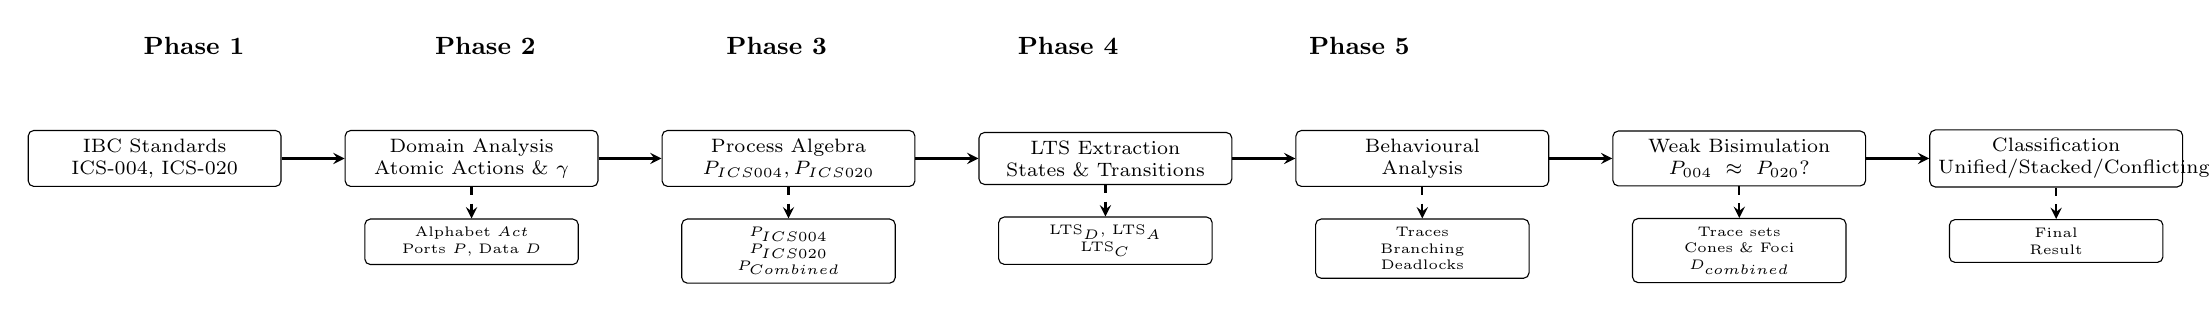
\begin{tikzpicture}[
    node distance=0.6cm and 0.8cm,
    box/.style={rectangle, draw, text width=3cm, align=center, 
                font=\scriptsize, inner sep=3pt, rounded corners=2pt},
    arrow/.style={->, thick, >=stealth},
    stage/.style={font=\bfseries\small, anchor=south}
]

% Stage labels
\node[stage] at (0.5, 1.2) {Phase 1};
\node[stage] at (4.2, 1.2) {Phase 2};
\node[stage] at (7.9, 1.2) {Phase 3};
\node[stage] at (11.6, 1.2) {Phase 4};
\node[stage] at (15.3, 1.2) {Phase 5};

% Row 1 (main flow)
\node[box] (A) {IBC Standards\\ICS-004, ICS-020};
\node[box, right=of A] (B) {Domain Analysis\\Atomic Actions \& $\gamma$};
\node[box, right=of B] (C) {Process Algebra\\$P_{ICS004}, P_{ICS020}$};
\node[box, right=of C] (D) {LTS Extraction\\States \& Transitions};
\node[box, right=of D] (E) {Behavioural\\Analysis};
\node[box, right=of E] (F) {Weak Bisimulation\\$P_{004} \approx P_{020}$?};
\node[box, right=of F] (G) {Classification\\Unified/Stacked/Conflicting};

% Arrows between main boxes
\draw[arrow] (A) -- (B);
\draw[arrow] (B) -- (C);
\draw[arrow] (C) -- (D);
\draw[arrow] (D) -- (E);
\draw[arrow] (E) -- (F);
\draw[arrow] (F) -- (G);

% Row 2 (detailed outputs below each phase)
\node[box, below=0.4cm of B, text width=2.5cm, font=\tiny] (Bdet) {Alphabet $Act$\\Ports $P$, Data $D$};
\node[box, below=0.4cm of C, text width=2.5cm, font=\tiny] (Cdet) {$P_{ICS004}$\\$P_{ICS020}$\\$P_{Combined}$};
\node[box, below=0.4cm of D, text width=2.5cm, font=\tiny] (Ddet) {LTS$_D$, LTS$_A$\\LTS$_C$};
\node[box, below=0.4cm of E, text width=2.5cm, font=\tiny] (Edet) {Traces\\Branching\\Deadlocks};
\node[box, below=0.4cm of F, text width=2.5cm, font=\tiny] (Fdet) {Trace sets\\Cones \& Foci\\$D_{combined}$};
\node[box, below=0.4cm of G, text width=2.5cm, font=\tiny] (Gdet) {Final\\Result};

\draw[arrow, dashed] (B) -- (Bdet);
\draw[arrow, dashed] (C) -- (Cdet);
\draw[arrow, dashed] (D) -- (Ddet);
\draw[arrow, dashed] (E) -- (Edet);
\draw[arrow, dashed] (F) -- (Fdet);
\draw[arrow, dashed] (G) -- (Gdet);

\end{tikzpicture}%
}
\caption{Conceptual Framework for IBC Behavioural Analysis (Five Phases)}
\label{fig:conceptual-framework}
\end{figure}

\section{Research Methodology}\label{research-methodology}

This research will employ a
\textbf{formal specification and analytical verification} design. The
methodology follows a top-down decomposition approach:

\begin{enumerate}
    \item Start with the IBC protocol standards (ICS-004, ICS-020) as the authoritative source of truth
    \item Decompose each standard into its constituent atomic actions and interaction patterns
    \item Translate these patterns into process algebra terms using the operators defined in Chapter 3
    \item Extract LTS models from the process algebra terms using SOS rules
    \item Analyse the LTS models to identify traces, branching structures, deadlocks, and synchronisation patterns
    \item Compare the asset and data behaviours using weak bisimulation and deadlock detection
    \item Classify the relationship as Unified, Stacked, or Conflicting
\end{enumerate}

\textbf{Tools to be used:}

\begin{itemize}
    \item Manual process algebra specification (ACP/CCS style notation)
    \item Manual LTS extraction and analysis (guided by SOS rules)
    \item Optional: Validation using process algebra toolset (mCRL2 or CADP) if available
\end{itemize}

\subsection{Phase 1: Domain Analysis and Atomic Action
Identification}\label{phase-1-domain-analysis-and-atomic-action-identification}

This phase addresses \textbf{Objective 1} and provides the foundation
for \textbf{RQ1}.

\begin{enumerate}
\item
  Decompose IBC Standards

  Obtain the authoritative IBC standards:

  \begin{itemize}
      \item ICS-004: Channel and Packet Semantics (data transport layer)
      \item ICS-020: Fungible Token Transfer (asset transfer layer)
  \end{itemize}

  Sources: Cosmos IBC documentation and specification repositories
  \citep{cosmos2024ibcintro} \citep{cosmos_ibc}.
\item
  Identify Communication Ports

  Define the set of communication ports \(P\) for IBC:

  \begin{itemize}
      \item \(p_{chainA}\): Port on source blockchain
      \item \(p_{chainB}\): Port on target blockchain
      \item \(p_{relayer}\): Port for off-chain relayer (internal, will be abstracted)
      \item \(p_{channel}\): Logical channel endpoint
  \end{itemize}
\item
  Define Data Types

  Define the set of data \(D\) for IBC packets:

  \begin{itemize}
      \item \(d_{packet}\): General packet payload (bytes, payload-agnostic)
      \item \(d_{asset}\): Asset transfer payload (amount, denomination, sender, receiver)
      \item \(d_{ack}\): Acknowledgement data (success/failure, optional return data)
      \item \(d_{channel\_id}\): Channel identifier
      \item \(d_{sequence}\): Packet sequence number
      \item \(d_{timeout}\): Timeout height and timestamp
  \end{itemize}
\item
  Define Atomic Actions

  Define the atomic actions for IBC:

  \textbf{Handshake actions (ICS-004):} \[
  \begin{aligned}
  & chan\_open\_init_{A}(id) \\
  & chan\_open\_try_{B}(id) \\
  & chan\_open\_ack_{A}(id) \\
  & chan\_open\_confirm_{B}(id)
  \end{aligned}
  \]

  \textbf{Packet actions (ICS-004):} \[
  \begin{aligned}
  & send\_packet_{A}(p,d) \\
  & recv\_packet_{B}(p,d) \\
  & ack_{B}(p,d_{ack}) \\
  & recv\_ack_{A}(p,d_{ack}) \\
  & timeout_{A}(p)
  \end{aligned}
  \]

  \textbf{Asset-specific actions (ICS-020):} \[
  \begin{aligned}
  & lock_{A}(asset) \\
  & burn_{A}(asset) \quad \text{(alternative to lock)} \\
  & mint_{B}(voucher) \\
  & verify\_proof_{B}(proof)
  \end{aligned}
  \]
\item
  Define Communication Function

  Define the communication function \(\gamma\) that pairs send and read
  actions:

  \[
  \begin{aligned}
  & \gamma(send\_packet_{A}(p,d), recv\_packet_{B}(p,d)) = c\_packet(p,d) \\
  & \gamma(ack_{B}(p,d_{ack}), recv\_ack_{A}(p,d_{ack})) = c\_ack(p,d_{ack}) \\
  & \gamma(chan\_open\_init_{A}(id), chan\_open\_try_{B}(id)) = c\_open(id) \\
  & \gamma(chan\_open\_ack_{A}(id), chan\_open\_confirm_{B}(id)) = c\_confirm(id)
  \end{aligned}
  \]

  Mismatched or isolated actions (send without matching read, or vice
  versa) are blocked by the encapsulation operator \(\partial_H\).
\item
  Deliverable

  A complete alphabet specification containing:

  \begin{itemize}
      \item Set of ports \(P\)
      \item Set of data types \(D\)
      \item Set of atomic actions \(Act = Act_{handshake} \cup Act_{packet} \cup Act_{asset}\)
      \item Communication function \(\gamma\)
      \item Set of internal actions \(I\) to be abstracted (relayer forwarding, proof verification)
  \end{itemize}
\end{enumerate}

\subsection{Phase 2: Process Algebra
Specification}\label{phase-2-process-algebra-specification}

This phase addresses \textbf{Objective 2} and completes \textbf{RQ1}.

\begin{enumerate}
\item
  Specify ICS-004 (Data Transport)

  Define the channel handshake process: \[
  Handshake = chan\_open\_init_{A} \cdot (chan\_open\_try_{B} \cdot chan\_open\_ack_{A} \cdot chan\_open\_confirm_{B} + TimeoutReject)
  \]

  Define the packet flow process: \[
  PacketFlow = send\_packet_{A} \cdot (recv\_packet_{B} \cdot ack_{B} \cdot recv\_ack_{A} + timeout_{A})
  \]

  Define the full channel process (recursive for multiple packets): \[
  Channel = Handshake \cdot (PacketFlow)^* \cdot Close
  \] where \((PacketFlow)^*\) denotes zero or more repetitions of
  PacketFlow, and \(Close\) terminates the channel.

  Define the complete IBC data transport system: \[
  IBC_{Data} = \partial_H( Chain_A \parallel Relayer \parallel Chain_B )
  \] where:

  \begin{itemize}
      \item \(Chain_A\) and \(Chain_B\) are blockchain processes running Channel
      \item \(Relayer\) forwards packets internally (modelled as \(\tau\) actions)
      \item \(\partial_H\) blocks unmatched send/read actions (requires handshake completion)
  \end{itemize}
\item
  Specify ICS-020 (Asset Transfer)

  Define the lock/burn process on source chain: \[
  LockProcess = lock_{A}(asset) \cdot verify\_lock_{A} \cdot packet\_prep
  \]

  Define the mint/claim process on target chain: \[
  MintProcess = verify\_proof_{B} \cdot mint_{B}(voucher) \cdot ack\_send
  \]

  Define the full asset transfer (wrapped in ICS-004 packet): \[
  AssetTransfer = LockProcess \cdot SendPacket \cdot MintProcess + Rollback
  \] where \(Rollback\) handles timeout or verification failure by
  unlocking the asset.

  Define the complete IBC asset transfer system: \[
  IBC_{Asset} = \partial_H( ChainA_{asset} \parallel Relayer \parallel ChainB_{asset} )
  \]
\item
  Specify Combined System (for Conflict Detection)

  To test for conflicts, define the parallel composition of asset and
  data flows over the same channels: \[
  IBC_{Combined} = \partial_H( (Chain_A \parallel ChainA_{asset}) \parallel Relayer \parallel (Chain_B \parallel ChainB_{asset}) )
  \]
\item
  Deliverable

  Complete process algebra specifications for:

  \begin{itemize}
      \item \(P_{ICS004}\) (data transport only)
      \item \(P_{ICS020}\) (asset transfer only)
      \item \(P_{Combined}\) (both running concurrently)
  \end{itemize}

  All specifications follow the syntax defined in Chapter 3 and will be
  included in the appendices.
\end{enumerate}

\subsection{Phase 3: LTS Extraction}\label{phase-3-lts-extraction}

This phase addresses \textbf{Objective 3} and \textbf{RQ2}.

\begin{enumerate}
\item
  Generate LTS from Process Terms

  Using the SOS rules defined in Chapter 3 (Section 3.6), generate the
  LTS for each process term:

  \textbf{Procedure:}

  \begin{enumerate}
      \item Start from the initial state of the process term
      \item For each state, examine all possible SOS rule applications
      \item For each applicable rule, derive the next state and transition label
      \item Add the new state to the set \(S\) and the transition to \(\rightarrow\)
      \item Repeat until no new states are reachable (fixpoint)
      \item Mark termination states as \(\checkmark\)
      \item Mark deadlock states (no outgoing transitions, not terminated) as \(\delta\)
  \end{enumerate}
\item
  Record LTS Properties

  For each LTS (\(LTS_{Data}\), \(LTS_{Asset}\), \(LTS_{Combined}\)),
  record:

  \begin{enumerate}
      \item \textbf{States (S):} List of all reachable states with unique identifiers
      \item \textbf{Transitions (→):} Labelled edges between states
      \item \textbf{Partial traces:} All finite sequences of observable actions
      \item \textbf{Completed traces:} Sequences ending in \(\checkmark\) or \(\delta\)
      \item \textbf{Branching points:} States with multiple outgoing transitions (choice points)
      \item \textbf{Deadlock states:} States with no outgoing transitions and not marked \(\checkmark\)
      \item \textbf{Synchronisation patterns:} Transitions labelled with communication actions \(c_p(d)\)
  \end{enumerate}
\item
  Visualise LTS

  Produce transition graphs for each LTS. Example structure for
  \(LTS_{Data}\):

  \begin{verbatim}
  State S0 (Initial) --chan_open_init_A--> S1
  State S1 --chan_open_try_B--> S2
  State S2 --chan_open_ack_A--> S3
  State S3 --chan_open_confirm_B--> S4 (Channel Open)
  State S4 --send_packet_A--> S5
  State S5 --recv_packet_B--> S6
  State S6 (Choice) --ack_B--> S7 or --timeout_A--> S8
  ...
  \end{verbatim}
\item
  Deliverable

  For each specification (\(P_{ICS004}\), \(P_{ICS020}\),
  \(P_{Combined}\)):

  \begin{itemize}
      \item Complete LTS with enumerated states and transitions
      \item Set of partial traces
      \item Set of completed traces
      \item Set of deadlock states (if any)
      \item Branching structure documentation
  \end{itemize}
\end{enumerate}

\subsection{Phase 4: Behavioural
Comparison}\label{phase-4-behavioural-comparison}

This phase addresses \textbf{Objectives 4 and 5} and answers
\textbf{RQ3}.

\begin{enumerate}
\item
  Compare Trace Sets

  Compute and compare trace sets: \[
  \begin{aligned}
  T_{data} &= Traces(P_{ICS004}) \\
  T_{asset} &= Traces(P_{ICS020}) \\
  \end{aligned}
  \]

  Check:

  \begin{enumerate}
      \item \(T_{data} \subseteq T_{asset}\)? (Are all data traces also asset traces?)
      \item \(T_{asset} \subseteq T_{data}\)? (Are all asset traces also data traces?)
      \item \(T_{data} = T_{asset}\)? (Are the trace sets identical?)
  \end{enumerate}

  \textbf{Interpretation:}

  \begin{itemize}
      \item If \(T_{data} = T_{asset}\) → possible Unified (but must check branching)
      \item If \(T_{data} \subset T_{asset}\) → possible Stacked
      \item If neither inclusion holds → likely Conflicting or behaviours fundamentally different
  \end{itemize}
\item
  Check Weak Bisimulation

  Apply the Cones and Foci methodology \cite{Fokkink2004} to determine
  if \(P_{ICS004} \approx P_{ICS020}\):

  \textbf{Procedure:}

  \begin{enumerate}
      \item Construct a state mapping function \(\phi\) from states of \(P_{ICS020}\) to states of \(P_{ICS004}\)
      \item For each state in \(P_{ICS020}\), identify the matching "focus" state in \(P_{ICS004}\)
      \item Prove that for each visible action, the branching structure is preserved
      \item Prove that \(\tau\) steps in one process can be matched by zero or more \(\tau\) steps in the other
  \end{enumerate}

  If \(\phi\) exists and all proof obligations are satisfied, then
  \(P_{ICS004} \approx P_{ICS020}\) (weak bisimilar).
\item
  Detect Conflicts

  Compute deadlock sets: \[
  \begin{aligned}
  D_{data} &= Deadlock(P_{ICS004}) \\
  D_{asset} &= Deadlock(P_{ICS020}) \\
  D_{combined} &= Deadlock(P_{ICS004} \parallel P_{ICS020})
  \end{aligned}
  \]

  Check if: \[
  D_{combined} \not\subseteq D_{data} \cup D_{asset}
  \]

  If YES, then new deadlocks appear only when asset and data behaviours
  run concurrently. For each new deadlock, document the trace that leads
  to it.
\item
  Assign Final Classification

  Apply the decision rules from Table 4.1:
\item
  Deliverable

  \begin{itemize}
      \item Trace inclusion relationships (with evidence)
      \item Weak bisimulation proof or disproof (with Cones and Foci mapping)
      \item Deadlock sets for all three processes
      \item Final classification: \textbf{Unified}, \textbf{Stacked}, or \textbf{Conflicting}
      \item If Conflicting: Documented traces leading to new deadlocks
  \end{itemize}
\end{enumerate}

\subsection{Phase 5: Documentation and
Reusability}\label{phase-5-documentation-and-reusability}

This phase addresses \textbf{Objective 6}.

\begin{enumerate}
\item
  Standardise Notation

  Legends for all process algebra symbols used:

  \begin{table}[h]
  \centering
  \begin{tabular}{|l|l|}
  \hline
  \textbf{Symbol} & \textbf{Meaning} \\
  \hline
  \(a\) & Atomic action \\
  \(\cdot\) & Sequential composition \\
  \(+\) & Alternative composition (choice) \\
  \(\parallel\) & Parallel composition \\
  \(\partial_H\) & Encapsulation (block actions in set \(H\)) \\
  \(\tau_I\) & Abstraction (rename actions in \(I\) to \(\tau\)) \\
  \(\tau\) & Silent (internal) action \\
  \(\delta\) & Deadlock \\
  \(\checkmark\) & Successful termination \\
  \(\gamma\) & Communication function \\
  \(s_p(d)\) & Send action on port \(p\) with data \(d\) \\
  \(r_p(d)\) & Read action on port \(p\) with data \(d\) \\
  \(c_p(d)\) & Communication action (synchronised send/receive) \\
  \(\approx\) & Weak bisimulation \\
  \(\leftrightarrow_{rb}\) & Branching bisimulation \\
  \hline
  \end{tabular}
  \caption{Process Algebra Notation Legend}
  \end{table}
\item
  Document Assumptions and Abstractions

  List of all abstractions made (from Scope and Limitations in Chapter
  1):

  \begin{enumerate}
      \item Cryptographic verification (Merkle proofs, light client sync) is abstracted as \(\tau\)
      \item Economic incentives (gas costs, slashing, liquidity constraints) are not modelled
      \item Relayer behaviour is abstracted as \(\tau\) (only observable effects are packet delivery)
      \item Only ICS-004 and ICS-020 are modelled; ICS-27 (Interchain Accounts) and ICS-31 (Interchain Queries) are excluded
      \item Security properties beyond observable behaviour (e.g., double-spending resistance) are not verified
      \item No empirical validation or live protocol execution is performed
  \end{enumerate}
\item
  Produce Reusable Specification

  Format the complete specification as an appendix with:

  \begin{itemize}
      \item Complete alphabet definition
      \item Complete process algebra terms for \(P_{ICS004}\), \(P_{ICS020}\), and \(P_{Combined}\)
      \item Communication function \(\gamma\) definition
      \item Encapsulation set \(H\) and abstraction set \(I\)
      \item Commentary explaining each part of the specification
  \end{itemize}

  This specification is designed to be reusable for:

  \begin{itemize}
      \item Future comparison with Polkadot XCM
      \item Future comparison with Axelar General Message Passing (GMP)
      \item Input to automated process algebra tools (mCRL2, CADP, or similar)
  \end{itemize}
\item
  Deliverable

  \begin{itemize}
      \item An appendix for complete and commented process algebra specification
      \item An appendix for the extracted LTS models (states and transitions)
      \item Documentation of assumptions for future researchers
  \end{itemize}
\end{enumerate}

\section{Validation and Quality
Criteria}\label{validation-and-quality-criteria}

Unlike empirical research, formal modelling research requires different
validation criteria.

\subsection{Correctness of
Formalisation}\label{correctness-of-formalisation}

\begin{itemize}
    \item \textbf{Face validity:} The process algebra specification is reviewed against ICS-004 and ICS-020 documents line by line. Every protocol action in the standards has a corresponding atomic action or process term in the specification.
    \item \textbf{Systematic mapping:} A mapping table documents how each IBC standard element translates to process algebra.
    \item \textbf{Expert review (if available):} A researcher with formal methods or blockchain interoperability expertise reviews the specification for accuracy.
\end{itemize}

\subsection{Completeness of LTS
Extraction}\label{completeness-of-lts-extraction}

\begin{itemize}
    \item \textbf{State space coverage:} The LTS includes all states reachable from the initial state via SOS rule application. No reachable state is omitted.
    \item \textbf{Termination handling:} All termination states (\(\checkmark\)) are correctly identified.
    \item \textbf{Deadlock detection:} All deadlock states are identified and documented.
\end{itemize}

\subsection{Reproducibility}\label{reproducibility}

\begin{itemize}
    \item The complete process algebra specification is provided in the appendices.
    \item Each step of LTS generation is documented (transition-by-transition)
    \item If tools are used (mCRL2, CADP), the input scripts and commands are included
    \item The methodology is described with sufficient detail for another researcher to replicate
\end{itemize}

\subsection{Limitations}\label{limitations}

\begin{itemize}
    \item \textbf{Abstraction may hide subtle bugs:} Cryptographic failures (e.g., Merkle proof forgery) are not modelled; economic attacks (e.g., relayer bribery) are not captured; timing-dependent issues may be lost in \(\tau\) abstraction
    \item \textbf{Manual LTS extraction:} Manual derivation may introduce human error (mitigated by systematic SOS application and cross-checking)
    \item \textbf{Scalability:} State explosion may occur for highly concurrent scenarios (mitigated by compositional analysis and abstraction)
    \item \textbf{No empirical validation:} Results are theoretical predictions, not guarantees about live IBC implementations
\end{itemize}

\section{Ethical Considerations}\label{ethical-considerations}

This research involves no human subjects, no personal data collection,
and no live blockchain interaction. The formal modelling and analysis
are conducted entirely on publicly available protocol specifications
(ICS-004, ICS-020). No economic or security risks are introduced as no
actual assets or live transactions are involved. Proper attribution is
given to IBC standard authors, process algebra pioneers, and all cited
researchers.

\section{Summary}\label{summary}

This chapter has presented the conceptual framework and methodology for
analysing IBC\textquotesingle s asset and data behaviours. The key
elements are:

\begin{itemize}
    \item \textbf{Conceptual framework:} Operational definitions of observable behaviour, traces, branching structure, and deadlock specifically for IBC; three analytical scenarios (Unified, Stacked, Conflicting) with formal criteria; conceptual diagram showing the analysis flow
    \item \textbf{Methodology:} Five phases: (1) domain analysis and atomic action identification, (2) process algebra specification, (3) LTS extraction, (4) behavioural comparison using weak bisimulation and deadlock detection, (5) documentation for reusability
    \item \textbf{Validation:} Correctness through face validity and systematic mapping; completeness through state space coverage; reproducibility through complete specification in appendix
\end{itemize}

%\include{chapters/results}
%\include{chapters/recommendations}
% \include{chapters/conclusion} may also be used

\appendix
   \chapter{Use of Generative AI}

\section{Brainstorming}
Since generative AI tools like ChatGPT can quickly provide answers, it was used to ask trends that are happening in the field of Blockchain. It was asked to provide recent published papers that were checked by the proponents. It would give several research titles with the authors and links. The proponents would look at each of them to ensure their legitimacy. Extraction of the content of the provided researches were not used as there was no guarantee that the AI would give correct results. Tasks like those are prone to hallucinations.  

Another usage was the creation of keywords that can be used to search for papers from the online databases found in the internet. This made the curation of papers easier and faster. This, however, did not replace the manual reading of the existing papers especially their RRL section to find keywords, know more about the topic, and look for possible mentioned references. 

\section{Research Proper}
During the writing of this paper, AI was used to automatically convert comma separated values into tables using latex syntax. This was done for convenience since the actual data was already created by the proponents. 

AI was also used in debugging error messages given by latex compiler during the compilation of the PDF format.
%    \include{appendices/reports}
%    \include{appendices/io}
%    \include{appendices/code}
%    \include{appendices/usersguide}

%\nocite{*}
\bibliographystyle{siam}
{
\singlespace
\bibliography{references}
}

%\begin{vita}

Juan N. Dela Cruz is BS Information Technology student of the Department of Computer Science at the Ateneo de Naga University.
\\
\\
Peter P. San Pedro is BS Information Technology student of the Department of Computer Science at the Ateneo de Naga University.
\\
\\
John J. San Juan is BS Information Technology student of the Department of Computer Science at the Ateneo de Naga University.
\\
\\
Maria Theresa F. Ni\~{n}o is BS Information Technology student of the Department of Computer Science at the Ateneo de Naga University.

\end{vita}

\end{document}
